% !Mode:: "TeX:UTF-8"
\documentclass{article}
% !Mode:: "TeX:UTF-8"
\usepackage[english]{babel}
\usepackage[UTF8]{ctex}
\usepackage{amsmath, amsthm, amssymb}

% Figure
\usepackage{graphicx}
\usepackage{float} %% H can fix the location
\usepackage{caption}
\usepackage[format=hang,singlelinecheck=0,font={sf,small},labelfont=bf]{subfig}
\usepackage[noabbrev]{cleveref}
\captionsetup[subfigure]{subrefformat=simple,labelformat=simple,listofformat=subsimple}
\renewcommand\thesubfigure{(\alph{subfigure})}

\usepackage{epstopdf} %% convert eps to pdf
\DeclareGraphicsExtensions{.eps,.mps,.pdf,.jpg,.png} %% bmp, gif not supported
\DeclareGraphicsRule{*}{eps}{*}{}
\graphicspath{{img/}{figure/}{../figure/}} %% fig directorys

%% \usepackage{pstricks} %% a set of macros that allow the inclusion of PostScript drawings directly inside TeX or LaTeX code
%% \usepackage{wrapfig} %% Wrapping text around figures

% Table
\usepackage{booktabs} %% allow the use of \toprule, \midrule, and \bottomrule
\usepackage{tabularx}
\usepackage{multirow}
\usepackage{colortbl}
\usepackage{longtable}
\usepackage{supertabular}

\usepackage[colorinlistoftodos]{todonotes}

% Geometry
\usepackage[paper=a4paper, top=1.5cm, bottom=1.5cm, left=1cm, right=1cm]{geometry}
%% \usepackage[paper=a4paper, top=2.54cm, bottom=2.54cm, left=3.18cm, right=3.18cm]{geometry} %% ms word
%% \usepackage[top=0.1cm, bottom=0.1cm, left=0.1cm, right=0.1cm, paperwidth=9cm, paperheight=11.7cm]{geometry} %% kindle

% Code
%% \usepackage{alltt} %% \textbf can be used in alltt, but not in verbatim

\usepackage{listings}
\lstset{
    backgroundcolor=\color{white},
    columns=flexible,
    breakatwhitespace=false,
    breaklines=true,
    captionpos=tt,
    frame=single, %% Frame: show a box around, possible values are: none|leftline|topline|bottomline|lines|single|shadowbox
    numbers=left, %% possible values are: left, right, none
    numbersep=5pt,
    showspaces=false,
    showstringspaces=false,
    showtabs=false,
    stepnumber=1, %% interval of lines to display the line number
    rulecolor=\color{black},
    tabsize=2,
    texcl=true,
    title=\lstname,
    escapeinside={\%*}{*)},
    extendedchars=false,
    mathescape=true,
    xleftmargin=3em,
    xrightmargin=3em,
    numberstyle=\color{gray},
    keywordstyle=\color{blue},
    commentstyle=\color{green},
    stringstyle=\color{red},
}

% Reference
%% \bibliographystyle{plain} % reference style

% Color
\usepackage[colorlinks, linkcolor=blue, anchorcolor=red, citecolor=green, CJKbookmarks=true]{hyperref}
\usepackage{color}
\def\red#1{\textcolor[rgb]{1.00,0.00,0.00}{#1}}
\newcommand\warning[1]{\red{#1}}

% Other
%% \usepackage{fixltx2e} %% for use of \textsubscript
%% \usepackage{dirtree}  %% directory structure, like the result of command tree in bash shell


% !Mode:: "TeX:UTF-8"
%+++++++++++++++++++++++++++++++++++article+++++++++++++++++++++++++++++++++
%customize the numbering of equation, to make it like section-subsection-equation style, for example,1-2-3
\makeatletter\@addtoreset{equation}{subsection}\makeatother
\renewcommand\theequation{%
\thepart\arabic{section}%
-\thepart\arabic{subsection}%
-\thepart\arabic{equation}%
}
%theorem
\newtheorem{definition}{D\'efintion} %% 整篇文章的全局编号
\newtheorem*{thmwn}{Thm} %% without numbers
\newtheorem{theorem}{Th\'eor\`eme}[section] %% 从属于section编号
\newtheorem{corollary}{Corollary}[theorem] %% 从属于theorem编号
\newtheorem{lemma}{Lemma}
\newtheorem{proposition}{Proposition}[section]
\newtheorem{example}{Example}
\newtheorem*{attention}{Attention}
\newtheorem*{note}{Note}
\newtheorem*{remark}{Remark}
\newtheorem{question}{Question}[section]
\newtheorem{problem}{Problem}
\newtheorem{fact}{Fact}


% Equation
\newcommand\lasteq{(\theequation)\ } %% use \lasteq to reference the last equation
\newcommand{\eqspace}{\hspace{0.5cm}}
\newcommand{\eqnote}[1]{\text{ #1 }} %% insert text in math mode being treated as normal text
\newcommand\mytop[2]{\genfrac{}{}{0pt}{}{#1}{#2}} %% generate a fraction but without the line

% Vecteur
\def\vecteur#1{(#1_1,~#1_2,~\ldots,~#1_n)}
\def\vector#1{#1_1,~#1_2,~\ldots,~#1_n}

% Set
\newcommand{\R}{\mathbb{R}} %% the real number set
\newcommand{\N}{\mathbb{N}}
\newcommand{\Z}{\mathbb{Z}}
\newcommand{\Q}{\mathbb{Q}}
\newcommand{\set}[1]{\{#1\}}
\newcommand{\stcomp}[1]{\overline{#1}} %% set complement

% Logic
\newcommand{\si}{\textrm{\ if }}
\newcommand{\sinon}{\textrm{ si non}}
\newcommand{\then}{\textrm{ then }}
\newcommand{\et}{\textrm{\ et }}
\newcommand{\ou}{\textrm{ ou }}
\newcommand{\non}{\textrm{non }}
\newcommand{\ssi}{si et seulement si }

% Math Operator
\newcommand{\fun}[1]{\textit{#1}}
\DeclareMathOperator{\arccot}{arcot}
\DeclareMathOperator{\arcth}{arcth}
\DeclareMathOperator{\arcsh}{arcsh}
\DeclareMathOperator{\arch}{arch}
\DeclareMathOperator{\ch}{ch}
\DeclareMathOperator{\dth}{th} %% \th already used
\DeclareMathOperator{\sh}{sh}
\DeclareMathOperator{\var}{var}
\DeclareMathOperator{\Ker}{Ker}
\DeclareMathOperator{\Img}{Img}

\newcommand*\laplace{\mathop{}\!\mathbin\bigtriangleup}
\newcommand*\dalambert{\mathop{}\!\mathbin\Box}
\newcommand{\grad}[1]{\nabla #1}
\newcommand{\gradien}[1]{\nabla #1}
\newcommand{\divergence}[1]{\nabla \cdot #1}
\newcommand{\rotationnel}[1]{\nabla \times #1}
\newcommand{\rot}[1]{\nabla \times #1}

\newcommand{\diag}[1]{\textit{diag}(#1)}
\newcommand{\mean}[1]{\overline{#1}}
\newcommand{\estimate}[1]{\hat{#1}}
\newcommand{\indep}{\!\perp\!\!\!\perp}
\newcommand{\nindep}{\not\!\perp\!\!\!\perp}
\newcommand{\norm}[1]{\left\Vert #1\right\Vert}
\newcommand{\obey}[1]{\thicksim{#1}}

\usepackage{xspace}
\newcommand{\ps}[2]{\ensuremath{\langle #1 , #2\rangle}\xspace} %% produit scalaire

%% quantique operators
\newcommand\ket[1]{|#1\rangle}
\newcommand\bra[1]{\langle #1|}
\newcommand\braket[3]{\langle#1|#2|#3\rangle}

% Symbol
\newcommand{\infinity}{\infty}


\begin{document}
\title{Introduction to algorithm \\Eric's Notes}
\author{Eric}
\maketitle
\newpage
\tableofcontents
\newpage

\section{课程简介及算法分析}
\subsection{Insertion sort}
Pseudocode
\begin{verbatim}
INSERTION-SORT(A)
1 for j ← 2 to length[A]  #1是第一个元素
2 	do key ← A[j] //将将要插入的数据保存下来
3 	//Insert A[j] into the sorted sequence A[1 _ j - 1].
4	 i ← j - 1
5	 while i > 0 and A[i] > key
6		 do A[i + 1] ← A[i]
7		 i ← i - 1
8	 A[i + 1] ← key
\end{verbatim}
\begin{figure}[htbp]
  \centering
  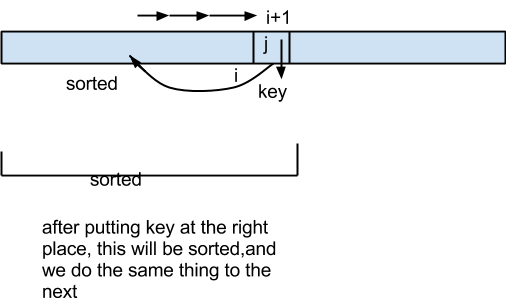
\includegraphics[scale = 0.7]{sort_insertion}\\
  \caption{Insertion sort}\label{fig.sort.insertion}
\end{figure}

ex:
\begin{verbatim}
8 2 4 9 3 6
2 8 4 9 3 6 // 2 goes before 8
2 4 8 9 3 6 // 4 goes before 8
2 4 8 9 3 6 // 9 stays there
2 3 4 8 9 6 // 3 goes before 4
2 3 4 6 8 9 // 6 goes before 8
\end{verbatim}

\begin{figure}[htbp]
  \centering
  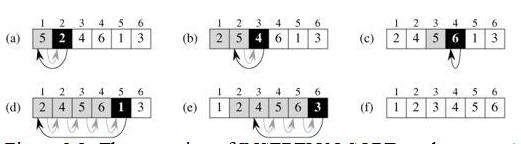
\includegraphics[scale = 0.7]{sort_insertion_example}\\
  \caption{Insertion sort}\label{fig.sort.insertion.example}
\end{figure}

python code
\begin{verbatim}
def insertionSort(L):
	#in place algorithem, 升序
	for j in range(1,len(L)):
		#将将要排序的数据保存下来, 开始对第j 个元素进行排序
		key=L[j]
		i=j-1
		#找到存放key的位置
		while i >= 0 and L[i]>key:
			L[i+1]=L[i] ## 将大数往后移动
			i=i-1
		##循环结束,说明L[i] <= key,所以key应该放在i+1处
		L[i+1]=key
	return L
\end{verbatim}

running time\\
1 already sorted: 最理想情况\\
2 reverse sorted: 最差情况

we want upper bounds 上界

kinds of analysis\\
worst-case $T(n)=$max time of any input of size n\\
average-case $T(n)=$expected time期望时间\\
(need assumption of statistical  distribution of inputs)\\
best-case (bogus假象)

BIG IDEA: \textbf{asymptotic analysis渐进分析}\\
not the the exact running time of an algorithm\\
the order of growth of the running time

the insertion sort analysis\\
worst-case: input reverse sorted
$$T(n)=\sum_{j=2}^{j=n} \theta(j)=\theta(n^2) \eqnote{算术级数arithmetic series}$$

\section{渐进符号,递归及解法}
\begin{definition}
\begin{figure}[htbp]
  \centering
  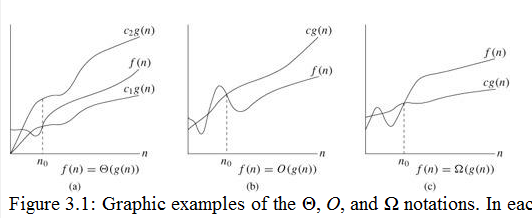
\includegraphics[scale = 0.7]{notation_asymptotical}\\
  \caption{Asymptotical notation}\label{fig.notation.asymptotical}
\end{figure}
\textbf{BIG O:上界 <=}\\
$O(g(n)) = \{f(n): $there exist positive constants $c$ and $n_0$ such that $0 \leq f(n) \leq cg(n)$ for all $n \geq n_0\}$\\
We say that $g(n)$ is an asymptotically upper bound for $f(n)$

\textbf{BIG $\Omega$下界 >=}\\
$\Omega(g(n)) = \{f(n): $there exist positive constants $c$ and $n_0$ such that $0\leq cg(n)\leq f(n)$ for all $n geq n_0\}$\\
We say that $g(n)$ is an asymptotically lower bound for $f(n)$.

\textbf{BIG $\Theta$ =}\\
$\Theta(g(n)) = \{f(n) : $there exist positive constants $c_1, c_2$, and $n_0$ such that $0\leq c\lg n\leq f(n)\leq c_2g(n)$ for all $n geq n_0\}$\\
$$\Theta(g(n))=O(g(n)) \cap \Omega(g(n)) $$\\
We say that $g(n)$ is an asymptotically tight bound for $f(n)$.

The definition of $\Theta(g(n))$ requires that every member $f(n) in \Theta(g(n))$ be asymptotically nonnegative, that is, that $f(n)$ be nonnegative whenever $n$ is sufficiently large.
\end{definition}

Ex:
$2n^2 + \Theta(n) = \Theta(n^2)$
for any function $f(n) in \Theta(n)$, there is some function $g(n) in \Theta(n^2)$ such that $2n^2 + f(n) = g(n)$ for all $n$. In other words, the right-hand side of an equation provides a coarser level of detail than the left-hand side.

o-notation
to denote an upper bound that is not asymptotically tight.\\
$o(g(n)) = \{f(n) : $for any positive constant $c > 0$, there exists a constant $n_0 > 0$ such that $0 \leq f(n) < cg(n)$ for all $n geq n_0\}$\\
For example, $2n = o(n^2)$, but $2n^2 \neq o(n^2)$

o-notation表示的是一种相差比较大的\\
in the o-notation, the function $f(n)$ becomes insignificant relative to $g(n)$ as $n$ approaches infinity; that is,
$$\lim_{n \to \infty} \frac{f(n)}{g(n)} = 0 $$

ω-notation
By analogy, ω-notation is to ?-notation as o-notation is to O-notation.
$$ \lim_{n \to \infty} \frac{f(n)}{g(n)} = \infty $$

\textbf{Comparison of functions}\\
与数的比较类比
\begin{itemize}
	\item $f(n) = O(g(n))	\approx	a \leq b$
	\item $f(n) = \Omega(g(n))	\approx a \geq b$
	\item $f(n) = \Theta(g(n))	\approx	a = b$
	\item $f(n) = o(g(n))	\approx	a \ll b$
	\item $f(n) = \omega(g(n))	\approx	a \gg b$
\end{itemize}

\subsection{Standard notations and common functions}
函数的单调性\\
monotonically increasing单调增\\
monotonically decreasing\\
strictly increasing严格递增\\
strictly decreasing

Floors and ceilings
$$
x -1 < \lfloor x \rfloor \leq x \leq \lceil x \rceil < x + 1
$$

For any integer $n, \lceil n/2 \rceil + \lfloor n/2 \rfloor = n$

And for any real number $n \geq 0$ and integer $a,b >0$
\begin{enumerate}
	\item $\lceil \lceil n/a \rceil /b \rceil = \lceil n/(ab) \rceil$
	\item $\lfloor \lfloor n/a \rfloor /b \rfloor = \lfloor n/(ab) \rfloor$
	\item $\lceil a/b \rceil \leq (a+(b-1))b$
	\item $\lfloor a/b \rfloor \geq (a-(b-1))/b$
	\item $a \mod n = a - \lfloor a/n \rfloor n$
\end{enumerate}

$\lim_{n \to \infty} \dfrac{n^b}{a^n} = 0$
from which we can conclude that
$n^b = o(a^n)$.
Thus, any exponential function with a base strictly greater than $1$ grows faster than any polynomial function.

$$
\lim_{n \to \infty} \frac{\lg ^b n}{(2^a)^{\lg n}} = \lim_{n \to \infty}\frac{\lg ^b n}{n^a} = 0
$$
$\lg^bn = o(n^a)$,
for any constant $a > 0$. Thus, any positive polynomial function grows faster than any polylogarithmic function.
$$
n! = \sqrt{2\pi n} (\frac{n}{e})^n (1 + \Theta(\frac{1}{n}))
$$
Functional iteration\\
We use the notation $f(i)(n)$ to denote the function $f(n)$ iteratively applied $i$ times to an initial value of $n$. Formally, let $f(n)$ be a function over the reals. For nonnegative integers $i$, we recursively define
$$
f^{(i)}(n) =
\left\{
  \begin{array}{ll}
		  n & \si i = 0\\
		  f(f^{(i-1)}(n)) & \si i >0
  \end{array}
\right.
$$
For example, if $f(n) = 2n$, then $f^{(i)}(n) = 2^in$.

\subsection{Substitution method}
Substitution method for solving recurrences entails two steps:\\
Guess the form of the solution.\\
Use mathematical induction(数学归纳法) to find the constants and show that the solution works.

Ex:
$T(n) = 2T(\lfloor n/2 \rfloor) + n$\\
猜测$T(n) = O(n \lg n)$,然后归纳法证明

$T(n) = 2T(n/2 + 17) + n$
与上一式相差$17$,但是当$n$很大时,$17$可以忽略掉,所以仍然猜测$T(n) = O(n \lg n)$,然后尝试用归纳法证明,发现是正确的

\subsubsection{Subtleties}
$T(n) = T(n/2) + T(n/2) + 1$.\\
我们猜测$T(n) \leq cn$\\
$T(n) \leq c n/2 + c n/2 + 1 =cn + 1$ ,wrong,但是只差了一个常数\\
we're only off by the constant 1, a lower-order term,加上一个lower-order term,猜测$T(n) \leq cn - b$\\
$T(n) \leq (c n/2 - b) + (c n/2- b) + 1 = cn - 2b + 1 \leq cn - b$\\
imply $b \geq 1$,所以当$b \geq 1$时,$T(n) \leq cn - b$

\subsubsection{Changing variables}
$T(n) = 2T(\lfloor \sqrt{n} \rfloor) +\lg n$\\
Renaming $m = \lg n$ yields  $T(2^m) = 2T(2^m/2) + m$.\\
We can now rename $S(m) = T(2^m)$ to produce the new recurrence
$S(m) = 2S(m/2) + m$,\\
这个见过,$S(m) = O(m \lg m)$.\\
Changing back from $S(m)$ to $T(n)$, we obtain
$$
T(n) = T(2^m) = S(m) = O(m \lg m) = O(\lg n \lg \lg n).
$$

\subsection{Recursion-tree method}
In a recursion tree, each node represents the cost of a single subproblem somewhere in the set of recursive function invocations.

We sum the costs within each level of the tree to obtain a set of per-level costs, and then we sum all the per-level costs to
determine the total cost of all levels of the recursion.

Recursion trees are particularly useful when the recurrence describes the running time of a divide-and-conquer algorithm.

A recursion tree is best used to generate a good guess,
which is then verified by the substitution method. So we can often tolerate a small amount of "sloppiness", since you will be verifying your guess later on.

Ex:
$T(n) = 3T(n/4) + \Theta(n^2)$\\
We create a recursion tree for the recurrence: $T(n) = 3T(n/4) + cn^2$,如图\ref{fig.compute.recursion_tree2}所示
\begin{figure}[htbp]
  \centering
  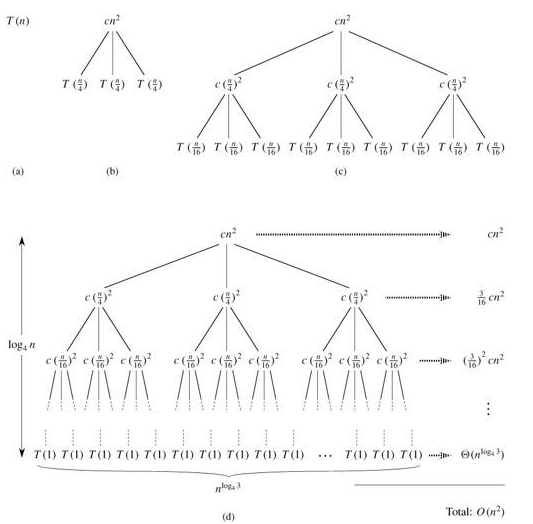
\includegraphics[scale = 0.7]{recursion_tree2}\\
  \caption{Recursion tree example}\label{fig.compute.recursion_tree2}
\end{figure}

Assume that n is an exact power of 4 (another example of tolerable sloppiness)\\
Its height is $\log_4 n$ (it has $\log_4 n + 1$ levels ($0, 1, 2,..., \log_4 n$))\\
The subproblem size for a node at depth i is $n/4^i$.\\
Each level has three times more nodes than the level above, and so the number of nodes at depth $i$ is $3i$.

深度为 $i = 0, 1, 2,..., \log_4 n - 1$,的nodes加起来 is $3^i c(n/4^i)^2 = (3/16)^icn^2$.\\
最后一层,at depth $\log_4n$, has $3^{\log_4 n} = n^{\log_4 3}$ nodes, each contributing cost $T(1)$, for a total cost of $n^{\log_4 3}T(1)$ , which is $\Theta(n^{\log_4 3})$.\\
把所有层的加起来,得到整个树的时间
\begin{equation}
\begin{split}
		T(n) & = cn^2 + \frac{3}{16} cn^2 + (\frac{3}{16})^2 cn^2 + \dots + (\frac{3}{16})^{\log_4 n - 1}cn^2 + \Theta(n^{\log_4 3}) \\
				   & = \sum_{i=0}^{\log_4 n - 1}(\frac{3}{16})^i cn^2 + \Theta(n^{\log_4 3}) \\
				   & = \frac{(3/16)^{\log_4 n} - 1}{(3/16)-1} cn^2 + \Theta(n^{\log_4 3})
\end{split}
\end{equation}
保留高阶项,得到$T(n)=O(n^2)$,
然后再用归纳法证明,发现是正确的

\subsection{Master method}
Theorem:Let $a \geq 1$ and $b > 1$ be constants, let $f(n)$ be a asymptotically positive function, and let $T(n)$ be defined on the nonnegative integers by the recurrence
$$T(n) = aT(n/b) + f(n)$$
Where we interpret $n/b$ to mean either $\lceil n/b \rceil$ or $\lfloor n/b \rfloor$. Then $T(n)$ can be bounded asymptotically as follows.
\begin{enumerate}
	\item If $f(n) = O(n^{\log_b a - \epsilon})$ for some constant $\epsilon > 0$, then $T(n) = \Theta(n^{\log_b a})$
	\item If $f(n) = n^{\log_{b} a}$, then $T(n) = \Theta(n^{\log_b a} \lg n)$
	\item If $f(n) = n^{\log_{b} a + \epsilon}$ for some constant $\epsilon > 0$, and if $a f(n/b) \leq cf(n)$ for some constant $c < 1$ and all sufficiently large $n$, then $T(n) = \Theta(f(n))$.
\end{enumerate}

总结规律如下:
Compare the function $f(n)$ with the function  $n^{\log_b a}$\\
if $f(n)$ is polynomial smaller, case $1$\\
if $f(n)$ is polynomial lager, case $3$

It is important to realize that \textbf{these three cases do not cover all the possibilities for} $f(n)$.
There is a gap between cases $1$ and $2$ when $f(n)$ is smaller than $n^{\log_b a}$ but not polynomially smaller.
Similarly, there is a gap between cases $2$ and $3$ when $f(n)$ is larger than $n^{\log_b a}$ but not polynomially larger.
If the function $f(n)$ falls into one of these gaps, or if the regularity condition in case $3$ fails to hold,
the master method cannot be used to solve the recurrence.

Ex: $T(n) = 3T(n/4) + n \lg  n$,\\
we have $a = 3, b = 4, f (n) = n \lg  n$,\\
$f(n)/(n^{\log_b a})=n\lg n/(n^{\log_4 3})=n^{1 - \log_4 3} \times \lg n$\\
so $f(n)$ is polynomial lager, case $3$, $T(n) = \Theta(n\lg  n)$.

\subsubsection{Proof of master method}
树的深度是$\log_b n$
图示证明见\ref{fig.compute.recursion_tree.proof}
\begin{figure}[htbp]
  \centering
  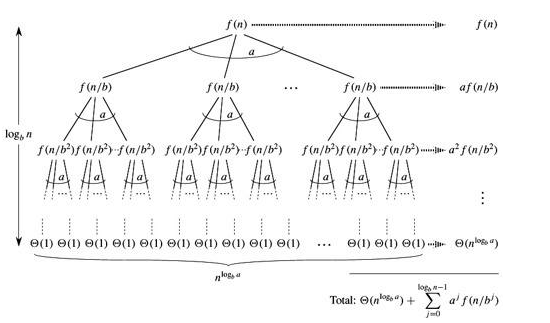
\includegraphics[scale = 0.7]{recursion_tree_proof}\\
  \caption{Recursion tree proof}\label{fig.compute.recursion_tree.proof}
\end{figure}
不太严格的证明,但是有助于理解\par
case 3:前面是呈几何级数递减的,所以前面所有层的和 is dominated by the first member $f(n)$\\
最后一层的和为$a^(\log_b n) \times  \Theta(1)=n^(\log_b a) \Theta(1)= \Theta(n^(\log_b a))$\\
$T(n)=\Theta(f(n))$\\
所以比较$f(n) and (n^(\log_b a))$也就是比较最后一层与前面所有层的

case 1:前面是呈几何级数递增的,因为$f(n)$ is polynomial smaller than $n^(\log_b a)$,所以整个求和中,$n^(\log_b a)$占据主导\\
$T(n)=\Theta(n^(\log_b a))$

case 2: 由于最顶层和最底层的差不多,在中间的,从最顶层呢过到最底层变化又不大,所以基本上都一个量级的,所以总和是:\\
$T(n)=(\log_b n+1)f(n)=(\log_b n+1) \times n^(\log_b a)=\Theta(f(n) \times \lg n)$

\section{快排及随机算法}
\subsection{Analysis}
当元素数目较少时,可以换用其他更快更直接的算法,这样可以避免再简单的情况下也进行递归\\
同时,这是一个tail recursion(尾递归),所以可以使用certain tail recursion optimizations

\textbf{worst-case time}\\
-input sorted or reverse sorted 元素都被分到了一边\\
so one side of partition has no elems, the other side has $n-1$ elems\\
每次递归只减少了$1$,所以递归次数非常多\\
$T(n)
= \Theta(n)+T(0)+T(n-1)
= \Theta(n) + \Theta(1)+T(n-1)
=T(n-1) + \Theta(n)$\\
式中$\Theta(n)$表示partition所需要的时间\\
使用递归树得到时间复杂度为:$T(n)=\Theta(n^2)$

\textbf{best-case analysis(intuition only!)}\\
if we are really lucky, partition splits array $n/2:n/2$\\
$T(n)=\Theta(n)+2T(n/2)=\Theta(n\lg n)$  和merge sort一样

\textbf{Partition $1/10:9/10$}\\
$T(n)=T(n/10)+T(9n/10)+\Theta(n)$\\
用递归树得到\\
$T(n)<=(\log_{10/9}n*cn)+\Theta(n)=O(n\lg n)$\\
$T(n)<=(\log_{10}n*cn)+\Theta(n)=\Omega(n\lg n)$\\
$T(n)=\Theta(n\lg n)$\\
The reason is that any split of constant proportionality yields a recursion tree of depth $\Omega(\lg n)$ whenever the split has constant proportionality.

Suppose we alternate \textit{lucky, unlucky, lucky}...\\
$L(n)=2U(n/2)+\Theta(n)$	lucky的后面是两个unlucky\\
$U(n)=L(n-1)+\Theta(n)$	unlucky\\
Then
$$
\begin{aligned}
L(n)
&=2U(n/2)+\Theta(n) \\
&=2(L(n/2 - 1) +\Theta(n/2))+\Theta(n)\\
&=2L(n/2 - 1) + \Theta(n)\\
&=\Theta(n\lg n)  \eqnote{lucky}
\end{aligned}
$$

Suppose we alternate \textit{unlucky, lucky, unlucky, lucky}...
$$
\begin{aligned}
U(n)
&=L(n-1) + \Theta(n) \\
&=[2U((n-1)/2) + \Theta(n)] +\Theta(n)\\
&=2U((n-1)/2)) + \Theta(n)\\
&=2U(n/2) + \Theta(n)\\
&=\Theta(n\lg n)  \eqnote{lucky}
\end{aligned}
$$

So when we alternate lucky, unlucky, lucky...,we are lucky\\
Or we alternate unlucky, lucky, unlucky, lucky..., we are luck too.\\
So how do we ensure that we are usually lucky? \\
Because if the input is already sorted or reverse sorted, we are going to be unlucky.\\
1.randomly arrange the elements\\
2.randomly choose the pivot

\subsection{Random quicksort}
pick the pivot randomly\\
选择好之后,把这个选中的与array的第一个元素交换位置,这样这个随机选择的pivot就到了array的第一位置,然后再运行Partition函数
\begin{itemize}
\item 运行时间不取决于输入数据的顺序
\item 对输入序列的分布不用做出假设
\item 不存在特定的输入序列会引起worst-case
\item worst-case determined only by random number generator
\end{itemize}

\subsection{Median-of-3 Pivot}
For example, the median-of-3 pivot approach selects three candidate pivots and uses the median one.
If the three pivots are chosen from the first, middle and last positions, then it is easy to see that for the already sorted array,
this will produce an optimum result: each partition will be exactly half ($\pm$ one element) of the problem and we will need exactly ceiling($\log n$) recursive calls.

\subsection{Random method analysis}
Random variable(随机变量) for running time assuming that random numbers are independent.\\
I want to know where I pivoted. 设这个pivot 的位置为随机变量$k$\\
So for $k=0, 1...n-1$ let\\
$x_k=1$ if partition generates a $k: n-k-1$ split, (pivot 算一个数, 所以两者加起来是n-1)\\
$x_k=0$ otherwise\\
这样一个partition,就产生了$n$个random variable,其中只有一个是$1$,其余的都是$0$.\\
例如如果产生的partition为$5:n-6$,那么只有$x_5=1,x_i=0 (i \in  [[0,n-1]]$ and $i!=5)$\\
this type of random variable is called \textbf{indicator random variable}

the expected value of $x_k:\\
E[x_k]=0*P(x_k =0)+1*P(x_k =1) = P(x_k =1) =1/n$\\
因为每一个数$k$ 都有可能取到, 而且概率是一样的, 所以每个数的概率都是 $1/n$
$$
T(n) =
\left\{
  \begin{array}{ll}
		  T(0) + T(n-1) \si 0:n-1 split \\
		  T(1) + T(n-2) \si 1:n-2 split \\
            \vdots \\
		  T(n-1) + T(0) \si n-1:0 split
  \end{array}
\right.
$$
所以这就是T(n)的递归,但是这个递归很麻烦,这里我们就可以看到indicator random variable的优美性,我们将使用indicator random variable将这个递归reduce to(规约到数学上)
$$
T(n) = \sum_{k=0}^{n-1} x_k (T(k) + T(n-k-1) + \Theta(n))
$$

$T(n)$的期望
\begin{equation}
\begin{split}
   E[T(n)] & =E[\sum_{k=0}^{n-1}x_k(T(k)+T(n-k-1)+\Theta(n))] \\
           & =\sum_{k=0}^{n-1}E[x_k(T(k)+T(n-k-1)+\Theta(n))]\\
           & \text{$x_k$随机变量独立于任何其他的partitions, 也就是说$x_k$ 区别于}\\
           & \text{其他递归调用,所以积的期望等于期望的积}\\
           & =\sum_{k=0}^{n-1}E[x_k]*E[(T(k)+T(n-k-1)+\Theta(n))]\\
           & = \frac{1}{n}\sum_{k=0}^{n-1}E[(T(k)] + \frac{1}{n}\sum_{k=0}^{n-1}E[T(n-k-1)] +\frac{1}{n}\sum_{k=0}^{n-1}\Theta(n)\\
           & =\frac{2}{n}\sum_{k=0}^{n-1}E[(T(k)] +\Theta(n)
\end{split}
\end{equation}

$x_k$ 是对$n$进行partition时产生的一个indicator random variable也就是说$x_k$是和$T(n)$ 是相关的, 而后面的$T(k)$ 与$T(n-k-1)$是在有了$x_k$ 之后, 也就是产生了一个$k,n-k-1$的分割后, 对产生的两个新的分割求时间时, 又会产生新的indicator: $x'_k$\\
所以$x_k$ 与$T(k), T(n-k-1)$是相互独立的, 可以运用概率的乘法原则

Absorb $k=0,1$ terms into $\Theta(n)$ for tech convenence,(两个常量加进去不影响$\Theta(n)$)
$$
E[T(n)]=\frac{2}{n}\sum_{k=2}^{n-1}E[T(k)]+\Theta(n)
$$

Use fact\todo{how to prove?}
$$
\sum_{k=2}^{n-1}k\lg k \leq \frac{1}{2}n^2\lg n-\frac{1}{8}n^2
$$
To prove $E[T(n)]<=a*n\lg n$ for constant $a>0$ with the substitution method\\
$E[T(n)] \leq an \lg n –bn (a, b >0)$\\
.....\\
所以我们得到$T(n)$的期望值是$\Theta(n\lg n)$\\
so the running time of randomized quicksort is $\Theta(n\lg n)$

The version of PARTITION given in this chapter is not the original partitioning algorithm. Here is the original partition algorithm, which is due to T.Hoare:
\begin{verbatim}
HOARE-PARTITION(A, p, r)
 1  x ← A[p]
 2  i ← p - 1
 3  j ← r + 1
 4  while TRUE
 5      do repeat j ← j - 1
 6           until A[j] <= x
 7         repeat i ← i + 1
 8           until A[i] >= x
 9         if i < j
10            then exchange A[i] with A[j]
11            else return j
\end{verbatim}
Every element of $A[p ‥ j]$ is less than or equal to every element of $A[j +1 ‥ r]$ when HOARE-PARTITION terminates.\\
The HOARE-PARTITION procedure always places the pivot value (originally in $A[p]$) into one of the two partitions $A[p ‥ j]$ and $A[j + 1 ‥ r]$.

\section{Heapsort}
Implementation of heap: tree or array\\
Max-heap: parent $\geq$ children,
	heapsort\\
Min-heap: parent $\leq$ children,
	priority queue

下面我们以Max-heap 进行讲解\\
Array n elements, leaves: $floor(n/2) + 1, floor(n/2) + 2, floor(n/2) + 3, \cdots, n$

The (binary) heap data structure is an array object that we can view as a nearly complete binary tree
\begin{verbatim}
PARENT(i)
   return floor(i/2)
LEFT(i)
   return 2i
RIGHT(i)
   return 2i + 1
\end{verbatim}

\begin{figure}[htbp]
  \centering
  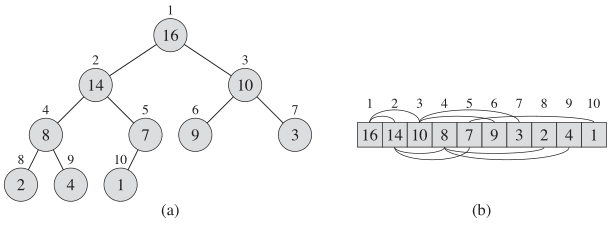
\includegraphics[scale = 0.7]{sort_heap_example}
  \caption{An example of heap}\label{fig.sort.heap.example}
\end{figure}

\noindent
The height of a node: the length of the longest downward path to a leaf from that node\\
The depth of a node: the length of the path to its root\\
Root node has depth 0, leaf node has height 0

\subsection{Maintaining the heap property}
Its inputs are an array A and an index i into the array\\
A[i] "float down"

\begin{verbatim}
Max-heapify(A, i)
   l = left(i)
   r = right(i)
   if l <= A.heap-size and A[l] > A[i]
      largest = l
   else largest = i
   if r <= A.heap-size and A[r] > A[i]
      largest = r
   if largest != i
      exchange A[i] with A[largest]
      Max-heapify(A, largest)
\end{verbatim}

max heapify: correct a single violation of the heap property in a sub tree's root\\
\textbf{运行Max-heapify(A, i) 的前提条件precondition}: assume that the trees rooted at left(i) and right(i) are max-heaps

\begin{figure}[htbp]
  \centering
  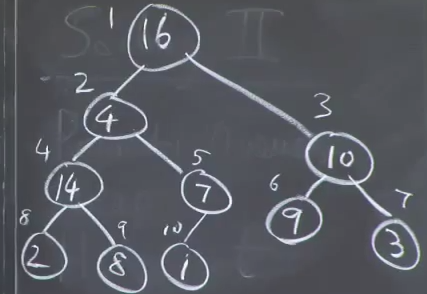
\includegraphics[scale = 0.7]{sort_heap_violation}
  \caption{An example of violation of heap property}\label{fig.sort.heap.violation}
\end{figure}
图\ref{fig.sort.heap.violation}中的第二个节点violates the max heap property, 所以我们可以调用max-heapify(A, 2), 修复好这个之后, 再进行检查直到不出现violation 为止

The children's subtrees each have size at most $2n/3$\todo{not understood}—the worst case occurs when the bottom level of the tree is exactly half full—and therefore we can describe the running time of MAX-HEAPIFY by the recurrence\\
$T(n) \leq T(2n/3) +\Theta(1)$\\
master theorem => $T(n) = O(\lg n)$

add a new item : place the new item at the last position(向左向下走知道不能继续前进), 然后进行修复, compare it with its parent, if it is larger than its parent, exchange them 向上继续进行这个比较直到不违反heap的性质, 也就是向上修复\\
delete the root : 将最后一个节点的值赋给root, 然后向下进行修复

\subsection{Building a heap}
build-max heap: produce a max heap from an unordered array

The elements in the subarray $A[(floor(n/2)+ 1)…n]$ are all leaves of the tree\todo{how to prove}\\
而leaf 已经是max-heap了, 因为leaf 没有children

The procedure BUILD-MAX-HEAP goes through the remaining nodes of the tree and runs MAX-HEAPIFY on each one
\begin{verbatim}
Build-Max-heap(A)
A.heap-size = A.length
    for i = floor(A.length / 2) downto 1
        Max-heapify(A, i) //每次调用max-heapify 之前, 都是满足max-heapify的precondition的
\end{verbatim}

Each call to MAX-HEAPIFY costs $O(\lg n)$ time, and BUILD-MAX-HEAP makes $O(n)$ such calls. Thus, the running time is $O(n\lg n )$. This upper bound, though correct, is not asymptotically tight.

但是我们可以发现:\\
max-heapify takes $O(1)$ for nodes that are one level above the leaves\\
and in general $O(l)$ time for nodes that re l levels above the leaves

an n-element heap has height $floor(\lg n )$ and at most $ceil(n/(2^{h+1}))$ nodes of any height $h$\todo{need proof}

$$
\sum_{h=0}^{\lfloor \lg n \rfloor} \lceil \frac{n}{2^{h+1}} \rceil O(h)
=
O(n \sum_{h=0}^{\lfloor \lg n \rfloor} \frac{h}{2^h})
$$

$$
\sum_{h=0}^{\infty} \frac{ h}{2^h} = \frac{1/2}{(1 - 1/2)^2} = 2
$$
Thus, we can bound the running time of BUILD-MAX-HEAP as
$$
O(n \sum_{h=0}^{\lfloor \lg n \rfloor} \frac{h}{2^h})
= O(n \sum_{h=0}^{\infty} \frac{h}{2^h})
= O(n)
$$

Hence, we can build a max-heap from an unordered array in linear time

\subsection{The heapsort algorithm}
build-max-heap from unordered array\\
find max element $A[1]$\\
swap elements $A[n]$ with $A[1]$, now max element is at the end of the array\\
Discard node $n$ from heap,\\
New root may violate max heap property, fix it

\begin{verbatim}
Heapsort(A)
    Build-Max-heap(A)
    for i = A.length downto 2
        exchange A[1] with A[i]
        A.heap-size = A.heap-size - 1
        Max-heapify(A, 1)
\end{verbatim}

把$A[1]$ 也就是最大值挪到最后一个位置, 同时将heap 的大小减一, 这样最大值就从heap 从取出来了并被放在了正确的位置上, 然后再修复这个heap; 然后再最大值重复这个操作

time $O(n\lg n )$\\
in place sort

\subsection{Priority queues}
max-priority queue, min-priority queue\\
we can use a heap to implement a priority queue

\begin{verbatim}
HEAP-MAXIMUM(A)
    return A[1]
\end{verbatim}
heap-maximum: $\Theta(1)$ time

\begin{verbatim}
HEAP-extract-MAX(A)
    if A.heap-size < 1
        error "heap underflow"
    max = A[1]
    A[1] = A[A.heap-size]
    A.heap-size = A.heap-size - 1
    MAX-HEAPIFY(A,1)
    return max
\end{verbatim}
heap-extract-max: $O(\lg n )$ time

\begin{verbatim}
HEAP-INCREASE-KEY(A,i,key)
    if key < A[i]
        error "new key is smaller than current key"
    A[i] = key
    while i > 1 and A[PARENT(i)] < A[i]
        exchange A[i] with A[PARENT(i)]
        i = PARENT(i)
\end{verbatim}
HEAP-INCREASE-KEY: $O(\lg n )$ time

\begin{verbatim}
MAX-HEAP-INSERT(A,key)
    A.heap-size = A.heap-size + 1
    A[A.heap-size] = -\infty
    HEAP-INCREASE-KEY(A,A.heap-size,key)
\end{verbatim}
MAX-HEAP-INSERT: $O(\lg n )$ time

\section{线性时间排序}
\begin{itemize}
\item quicksort $\Theta(n\lg n )$  randomized
\item heapsort $\Theta(n\lg n )$ 堆排序
\item merge sort $\Theta(n\lg n )$
\item insertion sort $\Theta(n^2)$
\end{itemize}

can we do better than $\Theta(n\lg n )$?\\
comparison sorting model\\
only use comparisons to determine relative order of elements

\subsection{decision tree model 决策树}
Ex: sort $<a_1, a_2, a_3>$

In general $<a_1,a_2...,a_n>$
\begin{itemize}
\item each internal node labeled $i, j$ means compare $a_i$ vs. $a_j$
\item left subtree $a_i <= a_j$
\item right subtree $a_i > a_j$
\item each leaf gives a permutation of the array
\end{itemize}

图\ref{fig.decision_tree.example}是一个决策树的例子
\begin{figure}[htbp]
  \centering
  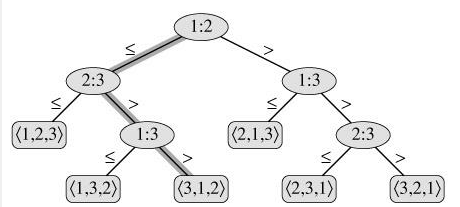
\includegraphics[scale = 0.7]{decision_tree_example}\\
  \caption{Decision tree example}\label{fig.decision_tree.example}
\end{figure}

\textbf{A lower bound for the worst case}\\
The length of the longest path from the root of a decision tree to any of its reachable leaves represents the worst-case number of comparisons. Consequently,
the worst-case number of comparisons for a given comparison sort algorithm equals the height of its decision tree. A lower bound on the heights of all decision trees in which each permutation appears as a reachable leaf is therefore a lower bound on the running time of any comparison sort algorithm. The following theorem establishes such a lower bound.

[Theorem 8.1] Any comparison sort algorithm requires $\Omega(n \lg n)$ comparisons in the worst case.\\
Proof: From the preceding discussion, it suffices to determine the height of a decision tree in which each permutation appears as a reachable leaf.\\
Consider a decision tree of height h with l reachable leaves corresponding to a comparison sort on n elements.
Because each of the $n!$ permutations of the input appears as some leaf, we have $n! \leq l$.(至少含有$n!$ 个leaves)
Since a binary tree of height h has no more than $2^h$ leaves, we have\\
$n! \leq l \leq 2^h$,
which, by taking logarithms, implies\\
$h \geq \lg (n!) = \Omega(n\lg n)$ (Stirling's approximation $n! \simeq (n/e)^n$

\subsection{Counting sort计数排序}
Element $\in [0, k]$ for some integer $k$. \\
When $k = O(n)$, the sort runs in $\Theta(n)$ time.\\
The \textbf{basic idea} of counting sort is to \textbf{determine, for each input element $x$, the number of elements less than $x$}.
This information can be used to place element $x$ directly into its position in the output array.\\
For example, if there are $17$ elements less than $x$, then $x$ belongs in output position $18$.
This scheme must be modified slightly to handle the situation in which several elements have the same value,
since we don't want to put them all in the same position.

input array $A[1,\ldots, n]$, and thus $length[A] = n$.\\
the array $B[1,\ldots,n]$ holds the sorted output, \\
the array $C[0,\ldots,k]$ provides temporary working storage.

\begin{verbatim}
COUNTING-SORT(A, B, k)
 1  for i ← 0 to k
 2     do C[i] ← 0
 3  for j ← 1 to length[A]
 4     do C[A[j]] ← C[A[j]] + 1
 5  // C[i] now contains the number of elements equal to i.
 6  for i ← 1 to k
 7     do C[i] ← C[i] + C[i - 1]
 8  // C[i] now contains the number of elements leqi
 9  for j ← length[A] downto 1
10     do B[C[A[j]]] ← A[j]
11        C[A[j]] ← C[A[j]] - 1
\end{verbatim}

An important property of counting sort is that it is \textbf{stable}.

Analysis\\
line $1-2 \Theta(k)$\\
line $3-4 \Theta(n)$\\
line $6-7 \Theta(k)$\\
line $9-11 \Theta(n)$\\
Overall time$\Theta(n+k)$\\
在实际上, 当 $k\Theta(n)$ 时, 我们才采用 counting sort

[Exercises 8.2-3] Suppose that the for loop header in line $9$ of the COUNTING-SORT procedure is rewritten as
\begin{verbatim}
9	 for j ← 1 to length[A]
\end{verbatim}
Show that the algorithm still works properly. Is the modified algorithm stable?\\
凭直觉来看, 不是stable

\subsection{Radix sort基数排序}
LSD(Least Significant Digit first)的基数排序适用于位数小的数列,如果位数多的话,使用MSD的效率会比较好.\\
MSD(Most Significant Digit first)的方式与LSD相反,是由高位数为基底开始进行分配,但在分配之后并不马上合并回一个数组中,
而是\textbf{在每个"桶子"中建立"子桶"},将每个桶子中的数值按照下一数位的值分配到"子桶"中.在进行完最低位数的分配后再合并回单一的数组中.

这里讲到的是LSD

\subsubsection{说明}
其原理在于对于待排序的数据,\textbf{整体权重未知}的情况下,
先按权重小的因子排序,然后按权重大的因子排序.\\
例如比较时间,先按日排序,再按月排序,最后按年排序,仅需排序三次.

但是如果先排序高位就没这么简单了.\\
\textbf{基数排序源于老式穿孔机,排序器每次只能看到一个列(这就是一个整体权重未知的例子)},
很多教科书上的基数排序都是对数值排序(这样意义不大),数值的大小是已知的,与老式穿孔机不同.将数值按位拆分再排序,是无聊并自找麻烦的事.算法的目的是找到最佳解决问题的方案,而不是把简单的事搞的更复杂.

\textbf{基数排序更适合用于对时间,字符串等这些整体权值未知的数据进行排序.}
这时候基数排序的思想才能体现出来,例如字符串,如果从高位(第一位)往后排就很麻烦.
而反过来,先对影响力较小,的低位(最后一位)进行排序就非常简单了.
这时候基数排序的思想就能体现出来.

$d$ 位数字, 每一位数字可以取 $k$ 个不同的数, 例如$0$ 到$9$ 十个数, 那么$k=10$
\begin{verbatim}
RADIX-SORT(A, d)
    for i from 1 to d:
        do use a stable sort to sort array A on digit i
\end{verbatim}

\subsubsection{Analysis}
time:$\Theta(d(n+k))$

证明:correctness\\
induct on digit position $t$\\
assume by induction 前$t-1$位已经排好序, 我们需要对第$t$位进行排序\\
1, if two elements have same t\textsuperscript{th} digit, stability $\Rightarrow$ same order $\Rightarrow$ sorted order\\
2, if different t\textsuperscript{th} digit $\Rightarrow$ sorted order

---use counting sort digits\\
---suppose we have $n$ integers each $b$ bits ( $range=[0,2^b-1]$, non-negative)\\
---split into $b/r$ "digits" each $r$ bits (将$r$个bits组合成一个大的"bit")\\
time $O(b/r*(n+k))=O(b/r*(n+2^r))$\\
对r求导, 令其为零求得此时的r值 $r=\lg n$\\
得到$O(bn/\lg n )$

if number in range $0,2^b-1$ then $time = O(dn)$\\
if  $d=O(1)$ then $time=O(n)$

而且只要$d$小于$\lg n$, 就可以击败comparison sort\\
但是在实际上, counting sort is not very good on a cache, in practice, radix sort is not that fast, unless your numbers are really small.\\
但是在理论上, 这个算法很优美

Finally, if you have arbitrary integers, that are one word length long, and you can manipulate a word in constant time.\\
Then the best algorithm we known for sorting runs $n*\sqrt{\lg\lg n }$, and this is a randomized algorithm and very complicated\\
有另外一个算法$n*lg(\lg n )$ worst case, 这篇论文应该可以看懂

\section{Hashing}
\subsubsection{Division method}
$h(k)=k \mod m$\\
When using the division method, we usually avoid certain values of $m$.\\
\red{一个数对$2^r$取余, 结果就是这个数的二进制表示的最后$r$位数字\\
同样的道理, 一个数对$10^r$取余, 结果就是这个数 的$10$进制表示的最后$r$位数字}\\
所以选择一个质数来作为$m$比较好, 这个质数一定不要接近$2$或者$10$的某个指数

\subsubsection{Multiplication method}
$h(k)=floor(m(kA\mod 1))$\\
where $x \mod 1$ mans the fractional part of $x$, that is $x - floor(x)$\\
$A$ is constant $\in (0,1)$

An advantage of the multiplication method is that the value of m is not critical. We typically choose it to be a power of $2$($m=2^p$ for some integer $p$). 这样multiplication method 就很容易在计算机上实现

\underline{具体执行方法}\\
word size of the machine: $w$ bits\\
$k$ fits into a single word\\
A is a fraction of the form $s/2^w$, where s is an integer in the range $0 < s < 2^w$. \\
we first multiply $k$ by the $w$-bit integer $s = A \cdot 2^w$. The result is a $2w$-bit value $r1*2^w + r0$, where $r1$ is the high-order word of the product and $r0$ is the low-order word of the product. \\
The desired $p$-bit hash value consists of the $p$ most significant bits of $r0$.\\
%% 这里有一个图片figure :D:\my-container\Documents\算法导论\figure\hash_multiplication_method.png\\
\begin{figure}[htbp]
  \centering
  % Requires \usepackage{graphicx}
  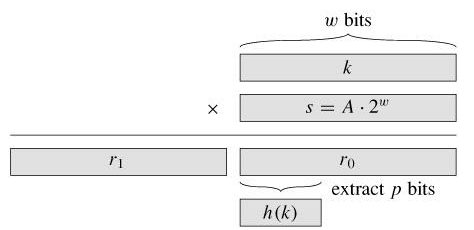
\includegraphics[width= 0.5\textwidth]{hash_multiplication_method}\\
  \caption{Multiplication method for Hash}\label{fig.hash.mult}
\end{figure}

Although this method works with any value of the constant A, it works better with some values than with others.\\
$A=(\sqrt{5} - 1)/2=0.6180339887$

\underline{Example}: suppose we have $k = 123456, p = 14, m = 2^{14} = 16384$, and $w = 32$. Adapting Knuth's suggestion, we choose $A$ to be the fraction of the form $s/232$ that is closest to , so that $A = 2654435769/232$. \\
Then $k \times s = 327706022297664 = (76300 \times 2^{32}) + 17612864$, \\
and so $r1 = 76300$ and $r0 = 17612864$\\
The $14$ most significant bits of $r0$ yield the value $h(k) = 67$\todo{14bits为什么只有67, 这么小??? 不知道这个是怎么算出来的}.\\
$17612864$的二进制表示为: $1000, 0110, 0110, 0000, 0010, 0000, 0$\\
$m=2^p$ and word size of machine is $w$-bit, \\
$k$ fits into a singl word\\
$h(k)=(A*k\mod 2^w) rsh (w-r)$\todo{这个是MIT视频教程中使用的方法}\\
A an odd integer in the range $(2^{w-r}-1, 2^w)$, don't pick $A$ too close to $2^{m-1}$ or $2^w$\\
rsh right shift

\section{Binary search tree(BST)}
Search trees are data structures that support many \textbf{dynamic-set operations}, including \textbf{search, minimum, maximum, predecessor前任, successor继承者, \red{insert, delete}}.\\
Thus, a search tree can be used both as a dictionay and as a priority queue.\\
These basic operations on a binary search tree take time proportional to the height of the tree.\\
所以, 对于complete binary tree with n nodes, these operations run in $\Theta(\lg n)$ worst-case.

\subsection{what is a binary seach tree?}
Each node is an object, \\
key field and satellite data, and left, right, p(parent) pointers.\\
if a child or parent is missing, the appropriate field contains the value NIL.

\underline{binary search tree property}\\
Let $x$ be a node in a binary search tree.\\
If $y$ is a node in the left subtree of $x$, then $key[y] \leq key[x]$.\\
If $y$ is a node in the right subtree of $x$, then $key[x] \leq key[y]$.\\
二叉排序树中,各结点关键字是惟一的.\\
注意:实际应用中,不能保证被查找的数据集中各元素的关键字互不相同,所以可将二叉排序树定义中BST性质(1)里的"小于"改为"小于等于",或将BST性质(2)里的"大于"改为"大于等于",甚至可同时修改这两个性质.\\

\subsubsection{tree walk 遍历}
\noindent Inorder tree walk 中序遍历\\
the key of the root of a subtree is printed between the values in its left subtree and those in its right subtree.\\
preorder tree walk: 前序遍历\\
postorder tree walk  后序遍历

\begin{verbatim}
Inorder-tree-walk(x):
    if x \neq nil:
        Inorder-tree-walk(left[x])
        print key[x]
        Inorder-tree-walk(right[x])
\end{verbatim}

it takes $\Theta(n)$ time to walk an n-node binary search tree.

\subsection{Querying a binary search tree}
search, minimum, maximum, successor, predecessor\\
all these operations $\Theta(h)$ time, where $h$ is the height of the binary search tree

\subsubsection{Searching}
递归式的
\begin{verbatim}
Tree-Search(x,k):
    if x=nil or k=key[x]
        return x
    if k < key[x]
        return Tree-Search(left[x], k)
    else return Tree-Search(right[x], k)
\end{verbatim}
执行的时候, x是root, 表示从root 开始search

迭代式的
\begin{verbatim}
Iterative-Tree-Search(x, k):
    while x != nil and k != key[x]
        if k<key[x]
            x=left[x]
        else x=right[x]
    return x
\end{verbatim}

\subsubsection{Minimum and maximum}
\noindent 一直往left subtree走就可以找到minimum\\
一直往right subtree走就可以找到maximum

\begin{verbatim}
Tree-Minimum(x):
while left[x] != nil
    x=left[x]
return x

Tree-Maximum(x):
while right[x] != nil
    x=right[x]
return x
\end{verbatim}

\subsubsection{Successor and predecessor}
successor 后继,
predecessor 前趋

\textbf{Successor} of a node x is the node with \textbf{the smallest key greater than $key[x]$}\\
A node's in-order successor is the left-most child of its right subtree\\
后继: 如果没有右子节点, 那么$x$ 的直接后继结点就是从$x$ 向上的路径中第一次右转时的节点

\textbf{Predecessor} of a node $x$ is the node with \textbf{the greatest key smaller than $key[x]$}\\
前趋: 如果没有左子节点, 那么$x$ 的直接前趋节点就是从$x$ 向上的路径中第一次左转时的节点\\
A node's in-order predecessor is the right-most child of its left subtree

某个节点有两个子女, 则其后继没有左子女, 其前趋没有右子女.\\
因为如果后继有左子女, 由于以后继为root的子树在那么左子女

The structure of a binary search tree allows us to determine the successor of a node \textbf{without ever comparing keys}.

\begin{verbatim}
Tree-Successor(x):
if right[x] !=nil
    return Tree-Minimum(right[x])
#当右子树非空时, the successsor is just the leftmost node in the right subtree

y=p[x]  # p is for parent
while y!=nil and x=right[y]
// 这里也可以分成两种情况, x 是p[x] 的left child 与 x 是p[x]的right child 两种情况
    x=y
    y=p[y]
return y
\end{verbatim}

\begin{figure}[htbp]
  \centering
  % Requires \usepackage{graphicx}
  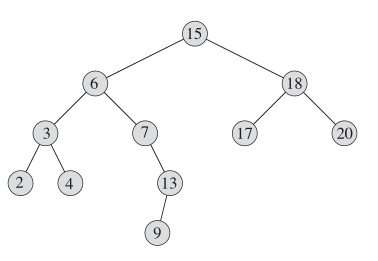
\includegraphics[scale = 0.7]{bst_example}\\
  \caption{Binary search tree example}\label{fig.bst.example}
\end{figure}

On the other hand, as Exercise 12.2-6 asks you to show, \\
if the right subtree of node is empty and $x$ has a successor $y$, then $y$ is the lowest ancestor of $x$ whose left child is also an ancestor of $x$. In Figure \ref{fig.bst.example}, the successor of the node with key 13 is the node with key 15. T\textbf{o find $y$, we simply go up the tree from $x$ until we encounter a node that is the left child of its parent}; this is accomplished by lines 3-7 of TREE-SUCCESSOR.

Tree-Predecessor is symmetric to Tree-Successor, both run in time $O(h)$

\subsection{Insertion and deletion}
\textbf{Insertion}\\
\begin{verbatim}
TREE-INSERT(T, z)
1  y ← NIL // 这个初始化时必须的, 因为当x一开始就是nil时, 就直接在line 9 对y==nil 进行判断
2  x ← root[T]
3  while x neq NIL
4      do y ← x
5         if key[z] < key[x]
6            then x ← left[x]
7            else x ← right[x]
8  p[z] ← y
9  if y = NIL
10     then root[T] ← z  # Tree T was empty
11     else if key[z] < key[y]
12             then left[y] ← z
13             else right[y] ← z
\end{verbatim}

\noindent line 4: 将$x$保存下来, 是因为while循环结束的时候, $x=nil$, 也就是现在$x$是叶子节点的子节点, 这个时候, $x$的parent就是一个叶子节点, 也就是说$y$是一个叶子节点, 而$z$ 将要成为$y$的一个子节点.\\
如果我们不把x的parent 保存下来, 一旦我们走到了一个leaf 处, 我们就没有办法把$z$ 放置到我们已经找到的位置.

\bigskip
\textbf{Deletion}\\
3 cases:\\
1, if z has \textbf{no children},见图\ref{fig.bst.deletion.case.1}, 直接删除掉z 就行了

\begin{figure}[htbp]
  \centering
  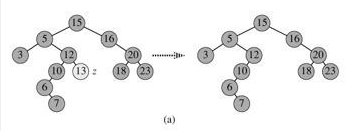
\includegraphics[scale = 0.7]{bst_deletion_case1}\\
  \caption{Case 1 of deletion}\label{fig.bst.deletion.case.1}
\end{figure}
%% figure:BST_delete_no_children\\

2, if $z$ has only \textbf{a single child}, 见图\ref{fig.bst.deletion.case.2},那么删除$z$, 将$z$ 的父节点与此孩子节点(子树) 关联就可以了
\begin{figure}[htbp]
  \centering
  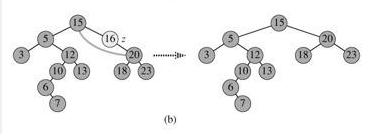
\includegraphics[scale = 0.7]{bst_deletion_case2}\\
  \caption{Case 2 of deletion}\label{fig.bst.deletion.case.2}
\end{figure}
%% figure: BST_delete_one_child

3, if $z$ has \textbf{two children},见图\ref{fig.bst.deletion.case.3}, 删除掉$z$ 的后继, 然后用$z$的后继来替代$z$\\
因为只有将$z$ 的后继放在$z$的位置, 才能够保持BST 的性质,$z$ 的后继由于是在$z$ 的右子树中的节点, 所以是大于$z$的左子树中所有的节点; 同时后继是右子树中最小的节点, 所以将这个后继挪到$z$的位置后, 是小于右子树中的所有节点\\
%% figure: BST_delete_two_children
\begin{figure}[htbp]
  \centering
  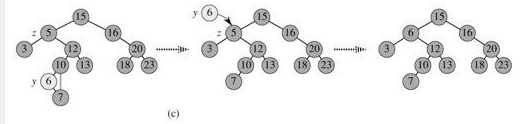
\includegraphics[scale = 0.7]{bst_deletion_case3}\\
  \caption{Case 3 of deletion}\label{fig.bst.deletion.case.3}
\end{figure}

我们可以将case 3 化为case 1和case 2两种已经解决的情况, 我们可以任意选取一个$z$的子树, 从底部开始, 把这个子树上所有的节点, 一个一个从树上摘下来, 存着, 然后$z$ 就成为一个只有一颗子树的节点, 然后就适用case 2. 删除完$z$ 后, 再把存着的那些节点重新插入到树上, 就完成了. 这个方法虽然有点笨, 但是确实是可行的.

其他办法: 要想不影响树的特性,那么最简单的想法是如果能只动$z$以及$z$以下的节点,那么树的其它部分肯定是OK的.那只要处理$z$以及$z$的子树就行了.想想,如果能在子树中找一个节点来替代$z$的位置,并保证新的子树也是满足二叉查找树要求的,这样改动量可能就比较小了.那么找哪个节点来代替它呢?当然是键值最接近X的,这样二叉树的特征就比较容易保持嘛.键值最接近$z$的,上面已经说过了,就是直接前趋和直接后继.正好,对于有两个子树的$z$来说,它的直接前趋和直接后继都是在它的子树中的,分别是左子树的最大值,右子树的最小值.而且,从子树中取下这两个节点(取下来干嘛?代替需要删除的X节点呗),也是比较容易的,因为"最大""最小"值节点,最多拥有不超过一个子节点(不然它绝对不够格做最大或最小).而没有子节点和只有一个子节点的节点删除,是我们已经会啦~~~.好,那么就\textbf{取前趋或后继就来代替需要删除的节点},问题就解决了.

\todo{这个代码不知道为什么不分三种情况来写, 非要写在一起, 看的就头疼, 还没有看懂}
\begin{verbatim}
TREE-DELETE(T, z)
1  if left[z] = NIL or right[z] = NIL
2      then y ← z
3      else y ← TREE-SUCCESSOR(z) //也可以用predeccessor
4  if left[y] neq NIL
5      then x ← left[y]
6      else x ← right[y]
7  if x neq NIL
8      then p[x] ← p[y]
9  if p[y] = NIL
10      then root[T] ← x
11      else if y = left[p[y]]
12              then left[p[y]] ← x
13              else right[p[y]] ← x
14  if y neq z
15      then key[z] ← key[y]
16           copy y's satellite data into z
17  return y
\end{verbatim}

\section{Augmenting data structures}
\subsection{Dynamic order statistics}
\noindent $select(x, i)$ return $i$\textsuperscript{th} smallest element in the subtree rooted at $x$\\
$rank(x)$ return the rank of a given element in the total ordering of the set\\
$size[x]$ which is the number of nodes in the subtree rooted at $x$.
\begin{figure}[htbp]
  \centering
  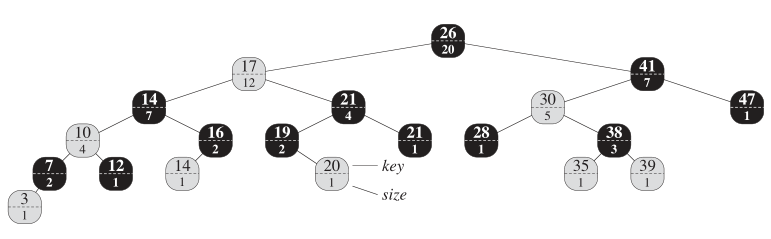
\includegraphics[scale =0.7]{order_statistics_tree}\\
  \caption{An order statistics tree}\label{fig.order_statistics_tree}
\end{figure}

\bigskip
An \textbf{order-statistic tree} $T$ is simply a red-black tree with additional information (size) stored in each node.\\
$size[x] = size[left[x]] + size[right[x]] + 1$\\
$size[nil] = 0$

\bigskip
在order-statistic tree中, 可以有相同的keys, 但是这样我们就需要重新定义一下rank\\
\textbf{rank}: the position at which it would be printed in an inorder walk of the tree.

\begin{verbatim}
OS-select(x, i)
    r = size[left[x]] + 1
    if i = r
        return x
    else if i<r
        return OS-select(left[x], i)
    else return OS-select(right[x], i - r)
\end{verbatim}

$O(\lg n)$ time

\begin{verbatim}
OS-RANK(T,x)
    r = size[left[x]] + 1
    y = x
    while y != root[T]
        if y = right[p[y]]
            r = r + size[left[p[y]]] + 1
        y = p[y]
    return r
\end{verbatim}

$O(\lg n)$ time

maintaining subtree sizes\\
刚开始的时候, 为一个干净的红黑树添加size, 需要$O(\lg n)$ time\\
在insert 和 delete 操作的时候, update size 是$O(1)$ 的操作, 因此insert 和 delete 仍然是 $O(\lg n)$ 的操作

\subsection{How to augment a data structure}
\underline{Theorem} 14.1 (\textbf{Augmenting a red-black tree})\\
Let f be an attribute that augments a red-black tree $T$ of $n$ nodes, and suppose that the value of $f$ for each node $x$ depends on only the information in nodes $x$, $x:left$, and $x:right$, possibly including $x:left:f$ and $x:right:f$. Then, we can maintain the values of $f$ in all nodes of $T$ during insertion and deletion without asymptotically affecting the $O(\lg n)$ performance of these operations.

\subsection{Interval tree}
这里我们研究的都是闭区间\\
Given a query interval, we can then quickly find an interval in the set that overlaps it

\textbf{interval trichotomy}\\
Any two intervals i and i' satisfy the interval trichotomy; that is, exactly one of the following three properties holds:
\begin{enumerate}
\item $i$ and $i'$ overlap,
\item $i$ is to the left of $i'$ (i.e., $high[i] < low[i']$),
\item $i$ is to the right of $i'$ (i.e., $high[i'] < low[i]$).
\end{enumerate}

we say that intervals $a$ and $b$ \textbf{overlap} if $a \cap b \neq \varnothing$ (Tex 中空集的表示方法),\\
that is if $low[a] \leq high[b]$ and $low[b] \leq high[a]$

Aninterval tree isared-black tree that maintains adynamic setof elements, with each element $x$ containing an interval $x:int$.

\noindent INTERVAL-INSERT(T, x)\\
INTERVAL-DELETE(T, x)\\
INTERVAL-SEARCH(T, i): returns a pointer to an element $x$ in the interval tree $T$ such that $int[x]$ overlaps interval $i$, or a pointer to the sentinel $nil[T]$ if no such element is in the set.
\begin{figure}[htbp]
  \centering
  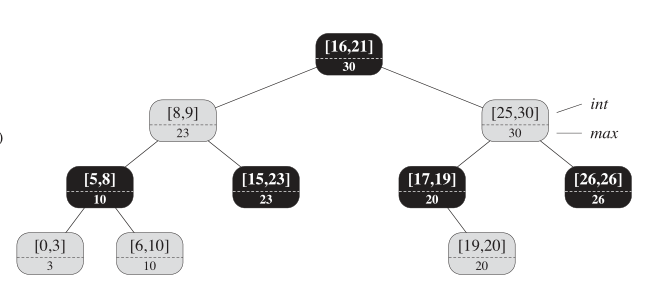
\includegraphics[scale =0.7]{interval_tree}\\
  \caption{An interval tree}\label{fig.interval_tree}
\end{figure}

\bigskip
\textbf{Underlying data structure}\\
We choose a red-black tree in which each node $x$ contains an interval $x:int$ and the key of $x$ is the low endpoint\\
\textbf{Additional information}\\
In addition to the intervals themselves, each node $x$ contains a value $x:max$, which is the maximum value of any interval endpoint stored in the subtree rooted at $x$\\
\textbf{Maintaining the information}\\
We must verify that insertion and deletion take $O(\lg n)$ time on an interval tree of n nodes. We can determine $x:max$ given interval $x:int$ and the max values of node $x's$ children:\\
$max[x] = max(high[int[x]], max[left[x]], max[right[x]])$\\
\textbf{Developing new operations}
\begin{verbatim}
INTERVAL-SEARCH(T, i)
    x = root[T]
    while x != nil[T] and i does not overlap int[x]
        if left[x] != nil[T] and max[left[x]] >= low[i]
            x = left[x]
        else x = right[x]
    return x
\end{verbatim}
也可以写成递归的形式, tail recursive call

\bigskip
\noindent list all overlapping intervals:\\
if $I$ have $k$ overlaps, then the time is $O(k\lg n)$\\
if $I$ search the second time, I get the same interval, so when I find one, delete it, and search agagin\\
output sensitive, 运行时间取决于输出结果

\bigskip
\noindent \underline{Theorem}: let $L = {i \in left[x]}, R = {i \in right[x]}$\\
1.if search goes right, then ${i' \in L, i' \eqnote{overlaps} i} = \varnothing$\\
2.if search goes left, then ${i' \in L, i' \eqnote{overlaps} i} = \varnothing => {i' \in R, i' \eqnote{overlaps} i} = \varnothing$\\
对于2. search goes left, 如果这时在左边没有找到overlaps, 那么我们也不可能在右边找到

\bigskip
segment tree

\section{Skiplist}
dynamic search structure, efficient, randomized, simple

\begin{figure}[htbp]
  \centering
  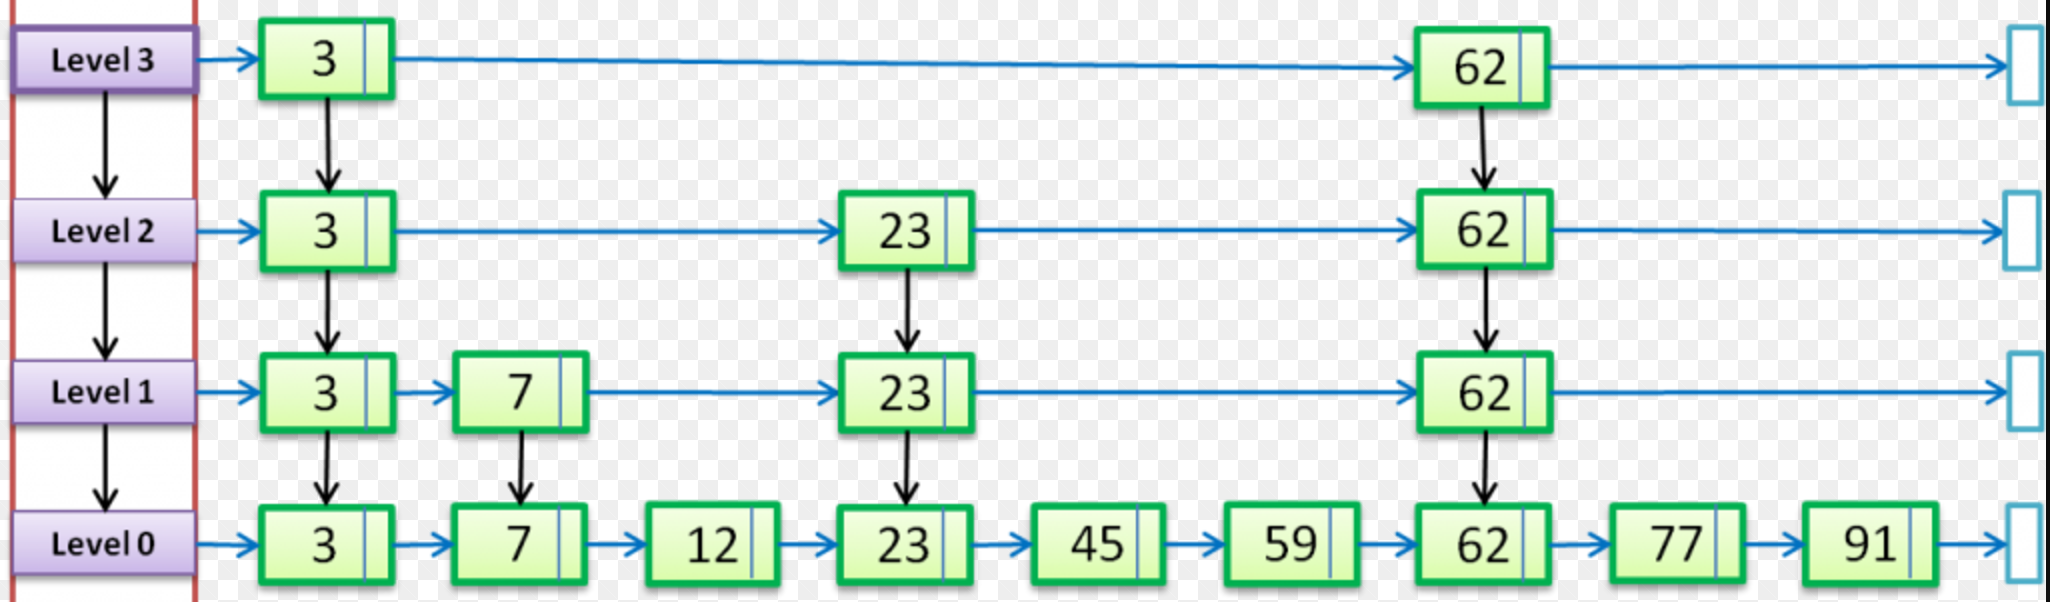
\includegraphics[scale =0.4]{skiplist}\\
  \caption{A skiplist}\label{fig.skiplist}
\end{figure}

对于一个sorted linked list, search 的复杂度为 $O(n)$, 因为虽然是有序的, 但是linked list 不能像数组那样随机访问, 还是需要遍历.

当在这个linked list 之上再加上一个linked list(level 1, 长度为$L_1$), 充当一个索引, 复杂度$\simeq L_1 + \dfrac{L_0}{L_1}$.
可以这么理解, 设想level 1 上的node 均匀的分布在level 0 的上面, 那么level 0 会被间隔为 $\dfrac{L_0}{L_1}$段.
通过level 1 上的node, 可以快速移动, 在level 0 上只需要移动其中的一段, 所以复杂度为$L_1 + \dfrac{L_0}{L_1}$.
当$L_1$ 为$\sqrt{L_0}$ 时, 复杂度取最小值$2 n^{1/2}$

当再加上level 2 时, 可以设想复杂度为 $3 n^{1/3}$

当一共有 $\lg n$ 个level 时, 复杂度为 $\lg n \times n^{1/\lg n}$, 即 $2 \lg n$

\noindent \underline{Lemma}:
number of lelvels in a $n$ element skiplist is $O(\lg n)$ with high probability($\simeq 1 - 1/(n^{\alpha})$)

Proof:

设$O(\lg n) = c \lg n$
$$
\begin{aligned}
\text{Failure probability}(not <= c \lg n \text{levels})
& = Pr(> c \lg n \text{levels}) \\
& = Pr(\text{the number of some element gets promoted} > c \lg n \text{times}) \\
& <= n \times Pr(\text{element x gets promoted} > c \lg n \text{times}) \\
& = n \times (1/2)^{c \lg n} \\
& = \dfrac{1}{n^{c - 1}} \\
& = \dfrac{1}{n^\alpha}
\end{aligned}
$$

\section{Dynamic programming}
optimal sub structure\\
a very powerful algorithmic paradigm in which a problem is solved by \textbf{identifying a collection of subproblems and tackling them one by one, smallest first, using the answers to small problems to help figure out larger ones, until the whole lot of them is solved}. \\
In dynamic programming we are not given a dag; the dag is implicit. Its nodes are the subproblems we define, and its edges are the dependencies between the subproblems: if to solve subproblem $B$ we need the answer to subproblem $A$, then there is a (conceptual) edge from $A$ to $B$. In this case, $A$ is thought of as a smaller subproblem than $B$\ ---\ and it will always be smaller, in an obvious sense.

Dynamic programming is effective when a given sub problem may arise from more than one partial set of choices; \textbf{the key technique is to store the solution to each such sub problem in case it should reappear}.\\
A dynamic programming algorithm will \underline{examine all possible ways} to solve the problem and will pick the best solution. Therefore, we can roughly think of dynamic programming as an intelligent, \underline{brute-force method} that enables us to go through all possible solutions to pick the best one. If the scope of the problem is such that going through all possible solutions is possible and fast enough, dynamic programming guarantees finding the optimal solution. The alternatives are many, such as using a greedy algorithm, which picks the best possible choice "at any possible branch in the road". While a \underline{greedy algorithm} does not guarantee the optimal solution, it is faster. Fortunately, some greedy algorithms (such as minimum spanning trees) are proven to lead to the optimal solution.

\underline{For example}, let's say that you have to get from point $A$ to point $B$ as fast as possible, in a given city, during rush hour. \\
A dynamic programming algorithm will look into the entire traffic report, looking into all possible combinations of roads you might take, and will only then tell you which way is the fastest. Of course, you might have to wait for a while until the algorithm finishes, and only then can you start driving. The path you will take will be the fastest one (assuming that nothing changed in the external environment). On the other hand, a greedy algorithm will start you driving immediately and will pick the road that looks the fastest at every intersection. \\
As you can imagine, this strategy might not lead to the fastest arrival time, since you might take some "easy" streets and then find yourself hopelessly stuck in a traffic jam.\\

\noindent
\textbf{Greedy algorithms}: make each choice in a locally optimal manner.\\
\textbf{Amortized analysis}: Instead of bounding the cost of the sequence of operations by bounding the actual cost of each operation separately, an amortized analysis provides a bound on the actual cost of the entire sequence. One advantage of this approach is that although some operations might be expensive, many others might be cheap.

We typically apply dynamic programming to \textbf{optimization problems}. Such problems can have many possible solutions. Each solution has a value, and we wish to \textbf{find a solution with the optimal (minimum or maximum) value}. We call such a solution an optimal solution to the problem, as opposed to the optimal solution, since there may be several solutions that achieve the optimal value.

When developing a dynamic-programming algorithm, we follow a sequence of four steps:
\begin{enumerate}
\item Characterize the structure of an optimal solution.
\item Recursively define the value of an optimal solution.
\item Compute the value of an optimal solution, typically in a bottom-up fashion.
\item Construct an optimal solution from computed information
\end{enumerate}

\subsection{Assembly-line scheduling}
 一个车间有2 条生产线, each assembly line with n stations, numbered by $j = 1, 2, 3, …,n$\\
$S_{i,j}$ the $j$\textsuperscript{th} station on assembly line $i$ ($i = 1$ or $2$)\\
$j$\textsuperscript{th} station on line 1 and $j$\textsuperscript{th} station on line 2 have the same function, but the time required varies.\\
assembly time on line $i$ at station $j$ is $a_{i , j}$\\
transfer time from line $i$ at station $j$ is $t_{i,j}$, $j = 1,2, … n-1$\\
enter time: $e_i$\\
exit time: $x_i$

\textbf{Step 1: the structure of the fastest way through the factory}\\
let us consider the fastest possible way for a chassis to get from the starting point through station $S_{1, j}$\\
if $j =1$, there is only one way\\
if $j=2,3,..n-1$, two ways, come from station $S_{1, j-1}$ and then directly to station $S_{1,j}$\\
or come from station $S_{2, j-1}$ and be transferred to station $S_{1, j}$

\textbf{Step 2: a recursive solution}\\
let $f_i[j]$ denote the fastest possible way to get a chassis from the starting point through station $S_{i,j}$\\
我们最终要求的是: 让一个chassis 最快速的通过这个组装线, we note it as $f^*$\\
$f^* = min(f_1[n] + x_1, f_2[n] + x_2)$

$$
\begin{aligned}
& f_1[1] = e_1 + a_{1,1}\\
& f_1[j] = min(f_1[j-1] + a_{1,j}, f_2[j-1] + t_{2, j-1} + a_{1, j} \si j \geq 2\\
& \\
& f_2[1] = e_2 + a_{2,1}\\
& f_2[j] = min(f_2[j-1] + a_{2,j}, f_1[j-1] + t_{1, j-1} + a_{2, j} \si j \geq 2\\
\end{aligned}
$$

\noindent
the $f_i[j]$ values give the values of optimal solutions to sub problems. To help us keep track of how to construct an optimal solution, let us define $l_i[j]$ to be the line number $i$($1$ or $2$), whose $j$\textsuperscript{th} station is used through the station $S_{i,j}$. here, $j=2,3,… n$\\
$l^*$ the line whose station $n$ is used\\
For example: $l^* = 1$, means we use station $S_{1,6}$\\
now we look at $l_1[6]$, which is $2$, means we use station $S_{2,5}$\\
now we look at $l_2[5]$, which is $2$, means we use station $S_{2,4}$\\
now we look at $l_2[4]$, which is $1$, means we use station $S_{1,3}$\\
now we look at $l_1[3]$, which is $2$, means we use station $S_{2,2}$\\
now we look at $l_2[2]$, which is $1$, means we use station $S_{1,1}$\\
这样我们就能够逆序追踪我们的最优解

\textbf{Step 3: Computing the fastest times}\\
如果直接计算, 类似于Fibonacci 数列的直接计算, 需要exponential time,\\
但是也同样类似于Fibonacci 数列, 后面的值只是取决于前面的值, 所以我们如果把前面已经计算出来的值保存下来, 每个$f$ 的计算都只需要常数的时间

\begin{verbatim}
FASTEST-WAY(a,t,e,x,n)
    f_1[1] = e_1 + a_{1,1}
    f_2[1] = e_2 + a_{2,1}
    for j = 2 to n:
        if f_1[j-1] + a_{1,j} <= f_2[j-1] + t_{2,j-1} + a_{1,j}
            f_1[j] = f_1[j-1] + a_{1,j}
            l_1[j] = 1
        else
            f_1[j] = f_2[j-1] + t_{2,j-1} + a_{1,j}
            l_1[j] = 2
        if f_2[j-1] + a_{2,j} <= f_1[j-1] + t_{1,j-1} + a_{2,j}
            f_2[j] = f_2[j-1] + a_{2,j}
            l_2[j] = 2
        else
            f_2[j] = f_1[j-1] + t_{1,j-1} + a_{2,j}
            l_2[j] = 1 //end for

    if f_1[n] + x_1 <= f_2[n] + x_2
        f^* = f_1[n] + x_1
        l^* =1
    else
        f^* = f_2[n] + x_2
        l^* =2
\end{verbatim}

\noindent
$\Omega(n)$ time

\textbf{Step 4: Constructing the fastest way through the factory}
\begin{verbatim}
PRINT-STATIONS(l,n)
    i = l^*
    print "line ",i,", station ",n
    for j = n downto 2
        i = l_i[j]
        print "line ",i,", station ",n
\end{verbatim}
这个打印是逆序的, 如果要正序输出, 可以采用recursive, 或者stack

\subsection{Longest common subsequence (LCS)}
Ex: longest common subsequence (LCS)
\begin{verbatim}
x : A B C B D A B
y : B D C A B A
\end{verbatim}
LCS: BDAB, BCAB, BCBA 都是长度为$4$, 没有长度为$5$

\bigskip
Analysis\\
check if a sequence is in $y:O(n), y$ is of length $n$\\
$2^m$ subsequences of $x$ ($x$ is of length $m$)\\
check all sub sequences of $x: O(n \cdot 2^m)$\\
exponential time = slow!

\bigskip
Simplification\\
1.look at the length of LCS(x,y)\\
2.Extend the alg to find LCS itself\\
Notation: $|s|$ denotes length of seq $s$\\
Strategy: consider \textbf{prefixs} of $x$ and $y$\\
Define $c[i,j] = |LCS(x[1… i], y[1…j])|$\\
Then, $c[m,n] = |LCS(x,y)|$\\
找出$c[i,j]$ 的通项公式

\bigskip
\underline{Theorem}:
$$
c[i,j] = c[i-1,j-1] + 1 if x[i] = y[j]
$$
$$
c[i,j] =max(c[i,j-1], c[i-1,j]) \eqnote{otherwise}
$$
\underline{Proof}:

\subsection{Fibonacci}
top-down approach
\begin{verbatim}
var m := map(0 → 0, 1 → 1)
   function fib(n)
       if map m does not contain key n
           m[n] := fib(n - 1) + fib(n - 2)
       return m[n]
\end{verbatim}
$O(n)$ time but requires $O(n)$ space
top-down approach 也可以减少空间的使用, 就是向bottom-up一样, 覆盖掉不用的值

\bigskip
bottom-up approach
\begin{verbatim}
function fib(n)
       if n = 0
           return 0
       var previousFib := 0, currentFib := 1
       else repeat n - 1 times  // loop is skipped if n=1
           var newFib := previousFib + currentFib
           previousFib := currentFib
           currentFib  := newFib
       return currentFib
\end{verbatim}
$O(n)$ time and requires $O(1)$ space\\
bottom-up 把previousFib 之前的都丢了, 所以可以减少空间的使用

\subsection{Optimal binary search trees}
might be compared with \textbf{Huffman trees}, which similarly seek to \textbf{place frequently used items near the root in order to produce a dense information encoding}; however, Huffman trees only store data elements in leaves and these elements need not be ordered.

\subsection{Common subproblems}
Finding the right subproblem takes creativity and experimentation. But there are a few standard choices that seem to arise repeatedly in dynamic programming.

i.The input is $x_1 ,x_2 ,\ldots ,x_n$ and a subproblem is $x_1,x_2,\ldots,x_i$ .\\
The number of subproblems is therefore linear.

ii.The input is $x_1,\ldots,x_n$ , and $y_1 ,\ldots ,y_m$ . A subproblem is $x_1 ,\ldots ,x_i$ and $y_1 ,\ldots ,y_j$ .\\
The number of subproblems is $O(mn)$.

iii.The number of subproblems is $O(mn)$.\\
The number of subproblems is $O(n2)$.

iv.The input is a rooted tree. A subproblem is a rooted subtree.\\
If the tree has n nodes, how many subproblems are there? exponential

\section{贪婪算法和最小生成树}
A greed algorithm always makes the choice that looks best at the moment. That is, it makes a locally optimal choice in the hope that this choice will lead to a globally optimal solution.

Dynamic programming usually solves the sub problems bottom up, a greedy algorithm usually progresses in a top-down fashion, making one greedy choice after another, reducing each given problem instance to a smaller one.

\subsection{Greedy versus dynamic programming}
The 0-1 knapsack problem:\\
Insolvable by greedy strategy, solvable by dynamic programming\\
Unable to fill the knapsack to capacity, and the empty space lowers the effective value per pound.

The fractional knapsack problem:\\
Solvable by greedy strategy, compute the value per pound $v_1/w_i$ for each item, take as much as possible of the item with the greatest value per pound.

\subsection{Tree}
\noindent
Graph: $E = O(V^2) \Rightarrow \lg E = O(\lg V)$  //省略绝对值的写法\\
digraph: directed graph\\
connected $\Rightarrow |E| > |V| - 1$: there is a path from any vertex to any other vertex in the graph.

adjacency matrix邻接矩阵 $n \times n$ matrix\\
where $V={1,2, … n}$\\
$A[i,j] = 1 \si (i,j) \in E$\\
$A[i,j] = 0 \si (i,j) \not \in E$
\begin{figure}[htbp]
  \centering
  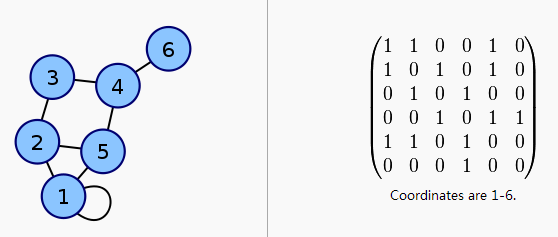
\includegraphics[scale = 0.7]{adjacency_matrix}\\
  \caption{Represent a graph with adjacency matrix}\label{fig.adjacency.matrix}
\end{figure}

Represent a graph with adjacency matrix, $O(V^2)$ storage $\Rightarrow$ dense representation\\
a complete graph, all elements are $1$

a sparse graph稀疏矩阵: 极端例子 a linked list
\begin{figure}[htbp]
  \centering
  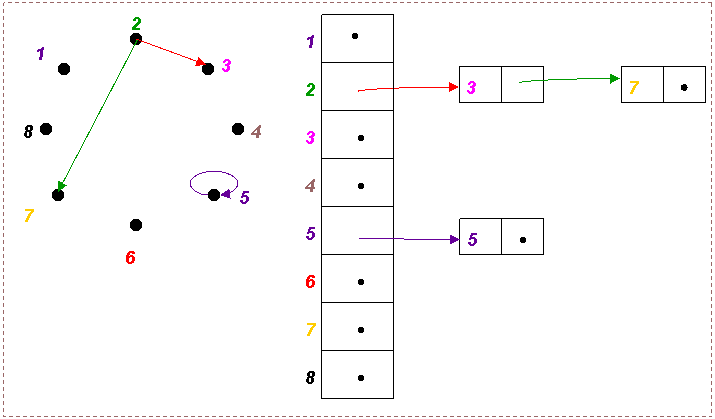
\includegraphics[scale = 0.6]{adjacency_list}\\
  \caption{Represent a graph with adjacency list}\label{fig.adjacency.list}
\end{figure}

Adjacency list\\
矩阵中每一行为1组成的一个list

\noindent
$|\mbox{Adj}[j]| =$ degree  if undirected graph\\
$|\mbox{Adj}[j]| =$ out degree  if directed graph

Handshaking Lemma (undirected graph)\\
$\sum_{v \in V} degree(v) = 2|E|$\\
每加入一条边, 这条边的两个顶点的degree 都增加$1$\\
For undirected graphs $\Rightarrow$ adjacency list uses $\Theta(V+E)$ storage

\subsection{Huffman code}
Huffman coding is a form of statistical coding.\\
Decoding: Once receiver has tree, it scans incoming bit stream, 0 means go left and 1 means go right.\\
Huffman coding is an entropy encoding algorithm used for lossless data compression.

\textbf{Huffman's paper: A method for the construction of minimum redundancy codes}

\textbf{Arithmetic coding and LZW coding}\\
\textbf{Linear time if input probabilities are sorted}

Uniform probability distribution and a number of members which is a power of two: Huffman coding is equivalent to simper binary block encoding, eg ASCII coding.

Shannon-Fano coding

A symbol with zero probability has zero contribution to the entropy.\\
$\lim_{p \to 0} p \cdot \log_{2} p = 0$

Entropy: the theoretical limit length established by Shannon.

A prefix code (sometimes called "prefix free codes") that is the bit string representing some particular symbol is never a prefix of the bit string representing another symbol.

\subsection{MST - Minimum spanning tress}
Distributed system\\
Input: connected, undirected graph $G=(V, E)$\\
$N: E \rightarrow R$ 权值\\
For simplicity, assume all edge weights are distinct $\Rightarrow N$ is injective\\
Output: A spanning tree $T$ (connects all vertexes) of minimum weight\\
	$W(T) = \sum_{(u, v) \in T} w(u, v)$ //$(u,v)$ is an edge

\begin{figure}[htbp]
  \centering
  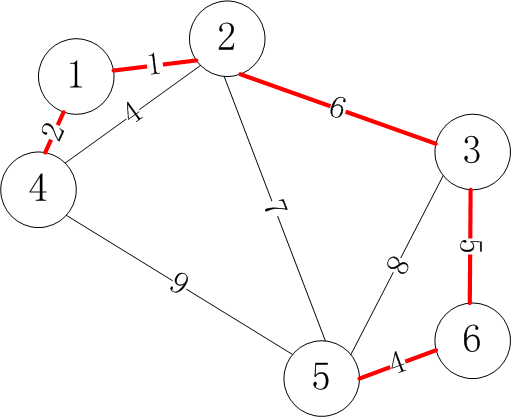
\includegraphics[scale = 0.5]{mst_result}\\
  \caption{红色是最小生成树的结果}\label{fig.mst.result}
\end{figure}

remove $(u, v)$ from $T$, then $T$ is partitioned into two sub trees $T_1$ and $T_2$\\

\noindent
\underline{Theorem}: $T_1$ is MST for $G_1 = (V_1, E_1)$ the sub graph of $G$ induced by vertexes in $T_1$\\
for $T_2$ the same thing\\
\underline{Proof}: cut and paste\\
$W(T) = W(u, v) + W(T_1) + W(T_2)$\\
if $\exists T'$ better than $T_1$ for $G_1$, then\\
overlapping sub problems? Yes\\
dynamic programming? Yes, but MST exhibits a better property $\Rightarrow$ greedy algorithm

\noindent
\underline{Theorem}: Let $T$ be MST of $G=(V, E)$, Suppose $(u,v)$ in $E$, least-weight edge connecting $A$ to $V-A$, then $(u,v)$ in $T$\\
\underline{Proof}: cut and paste

\section{Amortized Analysis}
\subsection{Incrementing a binary counter}
A k-bit binary counter that counts upward from $0$.\\
Use an array $A[0…k-1]$ of bits, where $A.length = k$, as the counter.\\
A binary number $x$ that is stored in the counter has its lowest-order bit in $A[0]$ and its highest-order bit in $A[1]$, so that $x=\sum_{i=0}^{k-1} A[i]*2^i$. Initially, $x = 0$
\begin{verbatim}
Increment(A)
    i = 0
    while i<A.length and A[i] == 1
        A[i] =0
        i = i + 1
    if i < A.length
        A[i] = 1
\end{verbatim}

A single execution of INCREMENT takes time $\Theta(k)$ in the worst case, in which array $A$ contains all $1$s. Thus, a sequence of $n$ INCREMENT operations on an initially zero counter takes time $O(nk)$ in the worst case.\\
We can tighten our analysis to yield a worst-case cost of $O(n)$ for a sequence of $n$ INCREMENT operations by observing that not all bits flip each time INCREMENT is called.\\
$A[0]$ does flip each time INCREMENT is called\\
$A[1]$, flips only every other time, flips $n/2$ times\\
Similarly, bit $A[2]$ flips only every fourth time, or $n/4$ times\\
bit $A[i]$ flips $n/(2^i)$ times in a sequence of $n$ INCREMENT operations on an initially zero counter.\\
For $i \geq k$, bit $A[i]$ does not exist, and so it cannot flip. The total number of flips in the sequence is thus
$$
\sum_{i=0}^{k-1}\lfloor \frac{n}{2^i} \rfloor
< n \sum_{i=0}^{\infty} \frac{1}{2^i}
= 2n
$$
The worst-case time for a sequence of $n$ INCREMENT operations on an initially zero counter is therefore $O(n)$. The average cost of each operation, and therefore the amortized cost per operation, is $O(n)/n = O(1)$
\subsection{Dynamic tables}
\begin{verbatim}
insert elements
     i	1	2	3	4	5	6	7	8	9 	10
size_i	1	2	4	4	8	8	8	8	16	16
cost_i	1	2	3	1	5	1	1	1	9 	1
\end{verbatim}

Cost of n inserts
$$
=\sum_{i=1}^n \mbox{cost}_i
=n+\sum_{j=0}^{\lfloor (\lg (n-1))\rfloor } 2^j
\leq 3n = \Theta(n)
$$
The average cost of a insert $= \Theta(n)/n=\Theta(1)$

\textbf{Amortized analysis}\\
Analyze a sequence of operations to show that average cost is small, even though 1 or serveral operations may be expensive\\
这里不涉及到概率分析

Types of amortized arguments\\
Aggregate (just saw)\\
accounting\\
potential

\subsection{Accounting method}
charge the $i$\textsuperscript{th} operation a fictitious amortized cost $c_i$ ($1$ pays for $1$ unit of operation)\\
fee is consumed to perform op\\
unused amount stored in bank for use in later ops

bank balance must not go negative:
$\sum_{i=1}^n \mbox{true-cost}_i \leq \sum_{i=1}^n \mbox{amortized-cost}_i$

\bigskip
Dynamic table\\
Charge $c_i = 3$\$ for $i$\textsuperscript{th} insert\\
\indent	1\$ pays for immediate insert\\
\indent	2\$ stored for table doubling\\
When table doubles\\
	\indent	1\$ moves recent item\\
	\indent	1\$ moves old item
\begin{verbatim}
0	0	0	0	2	2	2	2
\end{verbatim}
第五项插入时, 收取3\$, 其中1\$ 用于自己的插入, 剩下的2\$ 存入bank, 第$6, 7, 8$ 项插入时, 进行同样的操作, 这时银行刚好有8\$的存款\\
插入第$9$ 项时, table 需要double, 银行中剩余的8\$ 刚好可以支付原来$8$个elements 的移动到新table的花费
\begin{verbatim}
0	0	0	0	0	0	0	0	2
\end{verbatim}

Invariant bank balance $\geq 0$\\
$\sum_{i=1}^n \mbox{amortized-cost}_i =  3n$\\
实际上第一项可以只支付2\$, 从而可以省下1\$.

\subsection{Potential method}
Bank account viewed as potential energy of dynamic set

Framework
start with data structure $D_0$
op $i$ transforms $D_{i-1}$ to $D_{i}$

Define potential function\\
$\Phi: \{D\} \rightarrow R$ such that $\Phi(D_0) = 0$ and $\Phi(D) \geq 0$\\
Amortized cost $ac_i$ with respect $\Phi$ is\\
$ac_i = c_i + \Phi(D_i) - \Phi(D_{i-1})$\\
if $\Phi(D_i) - \Phi(D_{i-1})>0$ overcharge\\
if $\Phi(D_i) - \Phi(D_{i-1})<0$ undercharge
$$
\begin{aligned}
\sum_{i=0}^n ac_i
&= \sum_{i=0}^n (c_i + \Phi(D_i) - \Phi(D_{i-1}))
&= \sum_{i=0}^n c_i + \Phi(D_n) - \Phi(D_0)
&= \sum_{i=0}^n c_i + \Phi(D_n)
\end{aligned}
$$
我们需要$\sum_{i=0}^n ac_i \geq \sum_{i=0}^n c_i$, 所以应该保证$\Phi(D_n)\geq 0$, 但是实际上我们不知道应该怎样选择这样一个potential function, 所以我们通常保证$\Phi(D_i) \geq 0$

\textbf{Table doubling}\\
Define: $\Phi(D_i) = 2i – 2^{ceil(\lg i)}$\\
(Assume $2^{ceil(\lg 0)} = 0$)\\
Note: $\Phi(D_0) = 0$ and $\Phi(D_i) \geq 0$ (because $ceil(\lg i) = \lg i$ or $\lg i + 1$)\\
For example:
\begin{verbatim}
full	full	full	full	full	full		
\end{verbatim}
插入了$6$ 个, 此时 $\Phi = 2*6 – 2^{ceil(\lg 6)} = 12 – 8 =4$\\
如果我们用accounting method, 那么
\begin{verbatim}
0	0	0	0	2	2		
\end{verbatim}
此时bank balance 是$4$, 和上面的potential 一样\\
Amortized cost of $i$\textsuperscript{th} insert
$$
\begin{aligned}
ac_i
&= c_i +\Phi(D_i) - \Phi(D_{i-1})\\
&=
\left\{
  \begin{array}{ll}
		  i & \si i-1 \mbox{exact power of } 2\\
		  1 & \sinon
  \end{array}
\right.
+ (2i – 2^{ceil(\lg i)}) - (2(i-1) – 2^{ceil(\lg (i-1))})\\
&=
\left\{
  \begin{array}{ll}
		  i & \si i-1 \mbox{exact power of } 2\\
		  1 & \sinon
  \end{array}
\right.
+ 2 - 2^{ceil(\lg i)} + 2^{ceil(\lg (i-1))}
\end{aligned}
$$

Case 1: $i -1$ is exact power of $2$
$$
ac_i = i + 2 - 2^{ceil(\lg i)} + 2^{ceil(\lg (i-1))}
= i + 2 – 2^{\lg (i-1) + 1} + 2^{\lg (i-1)} = i + 2 – 2*(i-1) + (i-1) = 3
$$

Case 2: $i -1$ is not exact power of $2$\\
$ac_i = 1 + 2 - 2^{ceil(\lg i)} + 2^{ceil(\lg (i-1))} = 3$\\
$ceil(\lg i)$ 与$ceil(\lg (i-1)$ 是相等的\\

\textbf{Conclusions}\\
Amortized costs provide a clean abstraction for data structure performance.\\
Diff potential functions or accounting costs may yield diff bounds

\section{AVL tree}
\noindent
Self-balancing binary search tree

The heights of the two child subtrees of any node differ by at most one;

Time complexity in big $O$ notation
\begin{verbatim}
        Average  	Worst case
 Space	O(n)	       O(n)
Search	O(\log n)	O(\log n)
Insert	O(\log n)	O(\log n)
Delete	O(\log n)	O(\log n)
\end{verbatim}

Worst case is when right subtree has height  1 more than the left subtree for every node.

\noindent
$N_h$: min \# of nodes of height $h$\\
$N_h = 1+ N_{h-1} + N_{h-2}$\\
It looks like Fibonacci\\
$N_h > F_h = \frac{\phi^h}{\sqrt{5}}$ with $\phi = 1.618$  golden ratio\\
 $\frac{\phi^h}{\sqrt{5}} < n => h < c * \lg n$

\textbf{Insert}\\
1. simple BST insert\\
2. fix AVL property from changed node up

\textbf{AVL sort}\\
1. insert $n$ items - $\Theta(n\lg n)$\\
2. in-order traversal -$\Theta(n)$
\section{Graph}
We adopt a common notational convention: only inside asymptotic notation, such as $O$-notation, $\Theta$-notation, the symbol $V$ denotes $|V|$ and the symbol $E$ denotes $|E|$.

\noindent
The vertex set of a graph: $V[G]$\\
The edge set of a graph: $E[G]$

Sparse graph: $|E|$ is much less than $|V|^2$

\textbf{Breadth-first search: BFS}\\
Breadth-first search is so named because it expands the frontier between discovered and undiscovered vertices uniformly across the breadth of the frontier. That is, the algorithm discovers all vertices at distance $k$ from $s$ before discovering any vertex at distance $k+1$.

\bigskip
三种颜色的含义:\\
\textbf{White}: not having been discovered\\
\textbf{Gray}: frontier, discovered vertices that have not yet had their adjacency lists fully examined\\
\textbf{Black}: all its adjacency vertices have been examined

\noindent
$O(V+E)$ time

\bigskip
\textbf{Breadth-first trees}\\
The procedure BFS builds a breadth-first tree as it searches the graph, the tree is represented by the $\pi$ field in each vertex.\\
$G=(V, E)$ with source $s$\\
Predecessor subgraph of $G$ as $G\pi = (V\pi, E\pi)$, where\\
$V\pi = {v \in V: \pi[v] != NIL} {\cup s}$\\
$E\pi = {(\pi[v], v) : v \in V\pi - {s}}$

\section{最短路径算法}
Negative edge weight $\Rightarrow$ some shortest path may not exist.\\
Ex:\\
1.	图中出现了一个环, 而且这个环的总权值是负的negative cycle, 那么从u 到v的路径到达这个环时, 由于这个环的权值是负的, 它会永远地绕着这个环转下去, 使路径不断地变短\\
2.	$u$ 和$v$ 之间根本就没有路径

\textbf{optimal substructure}\\
a sub-path of a shortest path is shortest path.  // 用反证法 contradiction\\
Triangle inequality\\
$dist(u,v) \leq dist(u,x) + dist(x,v)$ //最短路径的定义\\
dist 表示最短路径

\textbf{Single source shortest path problem}\\
从源点$s$ 到所有其他点的最短路径\\
Assume all the edge weight are non-negative.\\
Idea: greedy

\subsection{Dijkstra's algorithm}
详细的可以看en wiki\\
a graph search algorithm that solves the single-source shortest path problem for a graph with non-negative edgepath costs, producing a shortest path tree. This algorithm is often used in routing and as a subroutine in other graph algorithms.\\
It picks the unvisited vertex with the lowest-distance, calculates the distance through it to each unvisited neighbor, and updates the neighbor's distance if smaller. Mark visited (set to red) when done with neighbors.

这里有一个图片(algo\_Dijkstra.gif),但是由于图片是gif 动态的, 无法放在这里
\begin{verbatim}
1  function Dijkstra(Graph, source):
2      for each vertex v in Graph:                                // Initializations
3          dist[v] := infinity ;     // Unknown distance function from source to v
5          previous[v] := undefined ;                // Previous node in optimal path
6      end for                                                    // from source
7
8      dist[source] := 0 ;                       // Distance from source to source
9      Q := the set of all nodes in Graph ; // All nodes in the graph are unoptimized –
                                                 //thus are in Q, priority queue
10    S: = empty set                  // no node optimized – thus S empty
11      while Q is not empty:                                      // The main loop
12          u := vertex in Q with smallest distance in dist[] ;    // Source node in first case
13          remove u from Q ;
14          if dist[u] = infinity:
15              break ;                                            // all remaining vertices are
16          end if                                                 // inaccessible from source
17          put u in S
18          for each neighbor v of u: //where v has not yet been removed from Q.
20              alt := dist[u] + dist_between(u, v) ;
21              if alt < dist[v]:                                  // Relax (u,v,a)
22                  dist[v] := alt ;
23                  previous[v] := u ;
24                  decrease-key v in Q;     // Reorder v in the Queue
                                       //因为v的距离被重新赋值了, 所以它在Q中的值也要相应地降低
25              end if
26          end for
27      end while
28      return dist;
29  end function
\end{verbatim}

Read the shortest path from source to target by reverse iteration
\begin{verbatim}
1  S := empty sequence
2  u := target
3  while previous[u] is defined:       // Construct the shortest path with a stack S
4      insert u at the beginning of S             // Push the vertex into the stack
5      u := previous[u]                           // Traverse from target to source
6  end while ;
\end{verbatim}

\noindent
Shortest path tree: the union of all shortest paths

breath first search: BFS 广度优先搜索\\
BFS 就是Dijkra\\

two changes\\
1. 不使用priority queue, 而是使用 FIFO queue\\
2. relax

\section{String matching}
The Rabin-Karp algorithm\\
String matching with finite automata\\
The Knuth-Morris-Pratt algorithm

\section{并行}
\noindent
parallel algorithms\\
dynamic multithreading\\
share memory, multicore
\begin{verbatim}
Ex: fib(n)
if n<2
    return n
x = spawn fib(n-1)
y = spawn fib(n-2)
sync
return (x+y)
\end{verbatim}
spawn: 衍生: Subroutine can execute at the same time with parent\\
Sync: wait until all children are done

\noindent
cashing

\section{Appendix}
\subsection{Summations}
harmonic series
$$H_n = 1+1/2+1/3+,\cdots,+1/n=\sum 1/k=\ln n + 0(1)
$$
\subsubsection{Approximation by integrals}
When a summation can be expressed as $\sum_{k=m}^n f(k)$, where $f(k)$ is a monotonically increasing function, we can approximate it by integrals:
$$
\int_{m-1}^n f(x)dx \leq \sum_{k=m}^n f(k) \leq \int_m^{n+1} f(x)dx
$$

\begin{figure}[htbp]
\begin{minipage}[t]{0.5\textwidth}
	\centering
	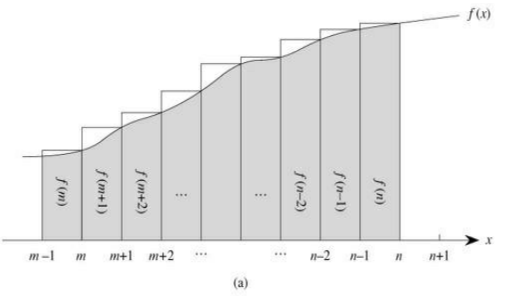
\includegraphics[width= \textwidth]{approximation_by_integrals_lower_bound}
  	\caption{approximation by lower bound}
  	\label{fig.approximation_by_integrals_lower_bound}
\end{minipage}
\begin{minipage}[t]{0.5\textwidth}
	\centering
	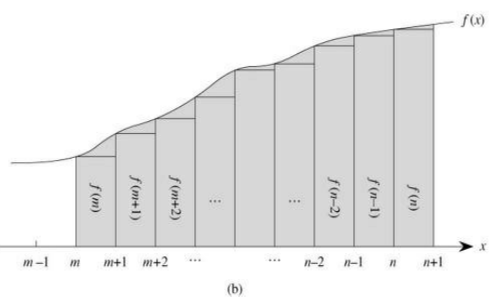
\includegraphics[width= \textwidth]{approximation_by_integrals_upper_bound}
  	\caption{approximation by upper bound}
  	\label{fig.approximation_by_integrals_upper_bound}
\end{minipage}
\end{figure}
when $f$ is monotonically decreasing function:
$$
\int_m^{n+1} f(x)dx \leq \sum_{k=m}^n f(k) \leq \int_{m-1}^n f(x)dx
$$
$n$\textsuperscript{th} harmonic number:
for a lower bound, we obtain
$$
\sum_{k=1}^n \frac{1}{k} \geq \int_1^{n+1}\frac{1}{x}dx = \ln(n+1)
$$

for the upper bound, we derive the inequality
$$
\sum_{k=2}^n \frac{1}{k} \leq \int_1^{n}\frac{1}{x}dx = \ln n
$$
which yields the bound
$$
\sum_{k=1}^n \frac{1}{k} \leq \ln n + 1
$$

\subsection{Relations}
A binary relation $R$ on two sets $A$ and $B$ is a subset of the Cartesian product $A \times B$
If $(a, b) \in R$, we sometimes write $a\ R\ b$. When we say that $R$ is a binary relation on a set $A$, we mean that $R$ is a subset of $A \times A$.

For example, the "less than" relation on the natural numbers is the set $\{(a, b) : a, b$ in $N$ and $a < b\}$.

An n-ary relation on sets $A_1, A_2,\ldots, A_n$ is a subset of $A_1 \times A_2 \times \cdots \times  A_n$.

A binary relation $R \subseteq A \times A$ is
\begin{description}
  \item[reflexive] if $a\ R\ b$ implies $b\ R\ a$ for all $a,b \in A$
  \item[symmetric] if $a\ R\ b$ implies $b\ R\ a$ for all $a, b \in A$. For example, "="
  \item[transitive] if $a\ R\ b$ and $b\ R\ c$ imply $a\ R\ c$ for all $a, b, c \in A$.
\end{description}

A relation that is reflexive, symmetric, and transitive is an equivalence relation

\bigskip
\begin{theorem}
\underline{An equivalence relation is the same as a partition} \\
The equivalence classes of any equivalence relation $R$ on a set $A$ form a partition of A, and any partition of $A$ determines an equivalence relation on $A$ for which the sets in the partition are the equivalence classes.
\end{theorem}

\bigskip
A binary relation $R$ on a set $A$ is antisymmetric if $a\ R\ b$ and $b\ R\ a$ imply $a = b$.

A relation that is reflexive, antisymmetric, and transitive is a partial order偏序.\\
And we call a set on which a partial order is defined a partially ordered set.\\
For example, the relation "is a descendant(子孙,后裔) of" is a partial order on these of all people (if we view individuals as being their own descendants).

In a partially ordered set A, there may be no single "maximum" element a such that $b\ R\ a$ for all $b \in A$. Instead, there may several maximal elements a such that for no $b \in A$, where $b \neq a$, is it the case that $a\ R\ b$. For example, in a collection of different-sized boxes there may be several maximal boxes that don't fit inside any other box, yet no single "maximum" box into which any other box will fit.

A partial order $R$ on a set $A$ is a total or linear order if for all $a, b \in A$, we have $a\ R\ b$ or $b\ R\ a$. That is, every pairing of elements of $A$ can be related by $R$.

1. The subset relation "$\subseteq$" on all subsets of $Z$ is a partial order but not a total order.

2. Give examples of relations that are
\begin{itemize}
	\item reflexive and symmetric but not transitive,
	\item reflexive and transitive but not symmetric,$\leq$
	\item symmetric and transitive but not reflexive.
\end{itemize}

\subsubsection{Functions}
Given two sets $A$ and $B$, a function $f$ is a binary relation on $A \times B$ such that $f$ or all $a \in A$,
there exists precisely one $b \in B$ such that $(a, b) \in f$

$f : A \rightarrow B$, \\
if $b = f(a), a$ is called the argument of $f$ and $b$ the value of $f$ at $a$.

When the domain of a function $f$ is a Cartesian product, we often omit the extra parentheses surrounding the argument of $f$.\\
eg, $f : A_1 \times A_2 \times \cdots \times A_n \rightarrow B$, we write $b = f(a_1,a_2,\ldots,a_n)$ instead of $b = f((a_1,a_2,\ldots,a_n))$. \\
We also call each $a_i$ an argument to the function $f$, though technically the (single) argument to $f$ is the n-tuple $(a_1,a_2,\ldots,a_n)$.\\
严格上来讲$(a_1,a_2,\ldots,a_n)$是一个参数

Give a bijection: $Z \rightarrow Z \times Z$.

\subsection{Graphs}
\textbf{Directed and undirected}\\
A directed graph (or digraph) $G$ is a pair $(V, E)$, where $V$ is a finite set and $E$ is a binary relation on $V$. \\
The set $V$ is called the $vertex顶点$ set of $G$, and its elements are called vertices (singular: vertex).\\
The set $G$ is called the edge set of $G$, and its elements are called edges.\\
In a directed graph, self-loops---edges from a vertex to itself are possible.\\
Vertices are represented by circles in the figure, and edges are represented by arrows

In an undirected graph $G = (V, E)$, the edge set E consists of unordered pairs of vertices, rather than ordered pairs.\\
In an undirected graph, self-loops are forbidden.

\bigskip
If $(u, v)$ is an edge in a directed graph $G = (V, E)$, we say that $(u, v)$ is incident from入射 or leaves vertex u and is incident to or enters vertex v.\\
If $(u, v)$ is an edge in an undirected graph $G = (V, E)$, we say that $(u, v)$ is incident on vertices u and v.\\
If $(u, v)$ is an edge in a graph $G = (V, E)$, we say that vertex v is adjacent 毗邻to vertex u.

The degree of a vertex in an undirected graph is the number of edges incident on it.\\
A vertex whose degree is $0$, such as vertex $4$ is isolated.

\bigskip
In a directed graph:\\
The out-degree of a vertex is the number of edges leaving it,\\
The in-degree of a vertex is the number of edges entering it.\\
The degree of a vertex in a directed graph is its in-degree plus its out-degree.

A path of length k from a vertex u to a vertex u' in a graph $G = (V, E)$ is a sequence $<v_0, v_1, \ldots, v_k>$of vertices such that $u = v_0, u' =v_k$, and $(v_{i-1}, v_i) \in E$ for $i = 1, 2,..., k$. \\
The length of the path is the number of edges in the path.

If there is a path p from u to u', we say that u' is reachable from u via p.\\
A path is simple if all vertices in the path are distinct.

\bigskip
In a directed graph, a path$<v_0, v_1, \ldots, v_k>$ forms a cycle if $v_0=v_k$  and the path contains at least one edge. \\
The cycle is simple if, in addition, $v_1, v_2,..., v_k$ are distinct. \\
A self-loop is a cycle of length $1$.

Two paths $<v_0, v_1, v_2, \ldots,v_{k-1}, v_0>$  and $<v'_0, v'_1, v'_2, \ldots,v'_{k-1}, v'_0>$ form the same cycle if there exists an integer j such that $v'_i=v_{(i+j) \mod k}$ for $i = 0, 1,..., k - 1$.\\
例如:\\
$v_0, v_1, v_2, v_3, v_4, v_0$\\
$v'_0, v'_1, v'_2, v'_3, v'_4, v'_0$\\
如果$v'_0 = v_3$, 那么\\
$v'_1=v_4=v_{1+3}$\\
$v'_2=v_{2+3}=v_5$ 但是实际上应该为$v_0$, 所以这里应该取{$(2+3) \mod5$}\\
$v'_3=v_{(3+3)\mod 5}=v_1$\\
$v'_4=v_{(4+3) \mod 5}=v_2$

A directed graph with no self-loops is simple. In an undirected graph, a path$〈v_0, v_1, \ldots, v_k〉$forms a (simple) cycle if $k \geq 3,v_0 = v_k$ and $v_1, v_2, \ldots, v_k$ are distinct.

A graph with no cycles is acyclic.

\bigskip
An undirected graph is connected if every pair of vertices is connected by a path. \\
The connected components of a graph are the equivalence classes of vertices under the "is reachable from" relation.\\
An undirected graph is connected if it has exactly one connected component, that is, if every vertex is reachable from every other vertex.

A directed graph is strongly connected if every two vertices are reachable from each other. The strongly connected components of a directed graph are the equivalence classes of vertices under the "are mutually reachable" relation. A directed graph is strongly connected if it has only one strongly connected component.

Two graphs $G = (V, E)$ and $G' = (V', E')$ are isomorphic if there exists a bijection $f : V \rightarrow V'$ \\
such that $(u, v) \in E$ if and only if $(f((u), f(v)) \in E'$.

In other words, we can relabel the vertices of $G$ to be vertices of $G'$, maintaining the corresponding edges in $G$ and $G'$.

\begin{figure}[htbp]
   \centering
   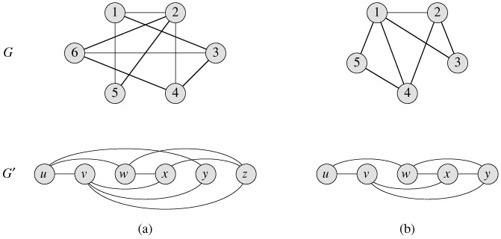
\includegraphics[scale = 0.7]{graph_isomorphic}\\
   \caption{graph isomorphic}\label{fig.graph.isomorphic}
 \end{figure}

$V = {1, 2, 3, 4, 5, 6}$ and $V' = {u, v, w, x, y, z}$. \\
Bijection $f(1) = u, f(2) = v, f(3) = w, f(4) = x, f(5) = y, f(6) = z$\\
图\ref{fig.graph.isomorphic}中a表示了一个\textbf{isomorphic}, b没有

\bigskip
Given an undirected graph $G = (V, E)$, the \textbf{directed version} of $G$ is the directed graph $G' = (V, E')$, where $(u, v) \in E'$ if and only if $(u, v) \in E$.

Given a directed graph $G = (V, E)$, the \textbf{undirected version} of $G$ is the undirected graph $G'= (V, E')$, where $(u, v) \in E'$ if and only if $u \neq v$ and $(u, v) \in E$.

In a directed graph $G = (V, E)$, a \textbf{neighbor} of a vertex $u$ is any vertex that is adjacent to $u$ in the undirected version of $G$ \\
That is, $v$ is a neighbor of $u$ if either $(u, v) \in E$ or $(v, u) \in E$. \\
In an undirected graph, $u$ and $v$ are neighbors if they are adjacent.

\bigskip
Several kinds of graphs are given special names. \\
A \textbf{complete graph} is an undirected graph in which every pair of vertices is adjacent. \\
A \textbf{bipartite双边 graph} is an undirected graph $G = (V, E)$ in which $V$ can be partitioned into two sets $V_1$ and $V_2$ such that $(u, v) \in E$ implies either $u \in V_1$ and $v \in V_2$ or $u \in V_2$ and $v \in V_1$. \\
That is, all edges go between the two sets $V_1$ and $V_2$.

An acyclic, undirected graph is a \textbf{forest},
and a connected, acyclic, undirected graph is a (free) \textbf{tree}. We often take the first letters of "directed acyclic graph"定向 非 循 环 图 and call such a graph a \textbf{dag}.

EX: Show that any connected, undirected graph $G = (V, E)$ satisfies $|E| \geq |V | - 1$.

\subsubsection{Trees}
A free tree is a connected, acyclic, undirected graph. We often omit the adjective "free" when we say that a graph is a tree. \\
If an undirected graph is acyclic but possibly disconnected, it is a forest.

Many algorithms that work for trees also work for forests.

\begin{figure}[htbp]
  \centering
  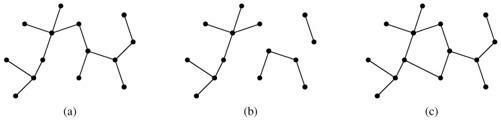
\includegraphics[scale = 0.7]{forest_and_tree}\\
  \caption{forest and tree}\label{fig.forest_and_tree}
\end{figure}

图\ref{fig.forest_and_tree}中a tree, b forest, c neither of them

\begin{theorem}
[Properties of free trees] Let $G = (V, E)$ be an undirected graph. The following statements are equivalent.
\begin{enumerate}
	\item $G$ is a free tree.
	\item Any two vertices in $G$ are connected by a unique simple path.
	\item $G$ is connected, but if any edge is removed from $E$ the resulting graph is disconnected.
	\item $G$ is connected, and $|E| = |V | - 1$.
	\item $G$ is acyclic, and $|E| = |V | - 1$.
	\item $G$ is acyclic, but if any edge is added to $E$ the resulting graph contains a cycle.
\end{enumerate}
\end{theorem}
\noindent
2中,unique 排除了cycle的存在, 因为如果有cycle, cycle中的两点间的path就不是unique\\
3中, edge移走后, 点还在\\
6中, 只增加edge, 而不增加点

\bigskip
A \textbf{rooted tree} is a free tree in which one of the vertices is distinguished from the others. The distinguished vertex is called the root of the tree. We often refer to a vertex of a rooted tree as a \textbf{node} of the tree.\\
Consider a node $x$ in a rooted tree $T$ with root $r$ \\
Any node $y$ on the unique path from $r$ to $x$ is called an \textbf{ancestor} of $x$ \\
If $y$ is an ancestor of x, then $x$ is a \textbf{descendant} of $y$ \\
(Every node is both an ancestor and a descendant of itself.) \\
If $y$ is an ancestor of $x$ and $x \neq y$, then $y$ is a \textbf{proper ancestor} of $x$ and $x$ is a \textbf{proper descendant} of $y$ The subtree rooted at $x$ is the tree induced by descendants of x, rooted at $x$

If the last edge on the path from the root $r$ of a tree $T$ to a node $x$ is $(y, x)$, then $y$ is the \textbf{parent} of x, and $x$ is a \textbf{child} of $y$ The root is the only node in $T$ with no parent. If two nodes have the same parent, they are \textbf{siblings}. A node with no children is an \textbf{external node or leaf}. A non leaf node is an \textbf{internal node}.

\bigskip
The number of children of a node $x$ in a rooted tree $T$ is called the \textbf{degree} of $x$

The length of the path from the root $r$ to a node $x$ is the \textbf{depth} of $x$ in $T$ \\
The \textbf{height} of a node in a tree is the number of edges on the longest simple downward path from the node to a leaf, \\
and the height of a tree is the height of its root.

\bigskip
An \textbf{ordered tree} is a rooted tree in which the children of each node are ordered. That is, if a node has $k$children, then there is a first child, a second child... and a $k$\textsuperscript{th} child.

\bigskip
\textbf{Binary and positional trees}\\
Binary trees are defined recursively. A \textbf{binary tree} $T$ is a structure defined on a finite set of nodes that either\\
\indent contains no nodes, or\\
\indent is composed of three disjoint sets of nodes: a \textbf{root} node, a binary tree called its \textbf{left} subtree, and a binary tree called its \textbf{right subtree}.\\

The binary tree that contains no nodes is called the empty tree or null tree, sometimes denoted NIL.

If the left subtree is nonempty, its root is called the \textbf{left child} of the root of the entire tree. Likewise, the root of a non null right subtree is the right child of the root of the entire tree.

\bigskip
\textbf{Full binary tree}\\
each node is either a leaf or has degree exactly $2$. There are no degree-1 nodes.

A $k$-ary tree is a positional tree in which for every node, all children with labels greater than $k$ are missing. \\
Thus, a binary tree is a $k$-ary tree with $k = 2$.\\
A complete k-ary tree is a $k$-ary tree in which all leaves have the same depth and all internal nodes have degree k.

How many leaves does a complete $k$-ary tree of height $h$ have? \\
The root has $k$ children at depth $1$, each of which has $k$ children at depth $2$, etc. \\
Thus, the number of leaves at depth $h$ is $k^h$. \\
Consequently, the height of a complete $k$-ary tree with $n$ leaves is $\log_k n$. The number of internal nodes of a complete k-ary tree of height $h$ is

$$
1 + k + k^2 + \cdots + k^{h-1} = \sum_{i=0}^{h-1} k^i = \frac{k^h - 1}{k-1}
$$

Thus, a complete binary tree $(k=2)$ has $2^h - 1$ internal nodes.
\begin{figure}[htbp]
  \centering
  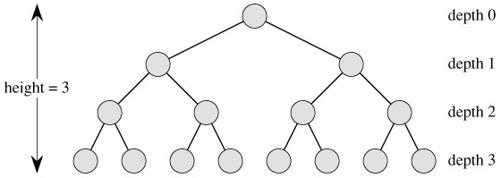
\includegraphics[scale = 0.7]{tree_height}\\
  \caption{tree height}\label{fig.tree.height}
\end{figure}

\bigskip
[Exercises B.5-3] Show by induction that the number of degree-$2$ nodes in any nonempty binary tree is $1$ less than the number of leaves.

[Exercises B.5-4] Use induction to show that a nonempty binary tree with $n$ nodes has height at least $\lg n$.

\subsection{Probability}
The conditional probability of an event $A$ given that another event $B$ occurs is defined to be.
在已知$B$发生的情况下, $A$发生的概率.
$$
Pr(A|B) = \dfrac{Pr(A \cap B)}{Pr(B)}
$$
whenever $Pr\{B\} \neq 0$. (We read "$Pr\{A | B\}$" as "the probability of $A$ given $B$.").
Intuitively, since we are given that event $B$ occurs, the event that $A$ also occurs is $A \cap B$. That is, $A \cap B$ is the set of outcomes in which both $A$ and $B$ occur.
Since the outcome is one of the elementary events in $B$, we normalize the probabilities of all the elementary events in $B$ by dividing them by $Pr\{B\}$, so that they sum to $1$.

\bigskip
Two events are \textbf{independent} if $Pr(A \cap B) = Pr(A)\cdot Pr(B)$ \\
which is equivalent, if $Pr\{B\} \neq 0$, to the condition $Pr\{A | B\} = Pr\{A\}$.
也就是说$A$的发生与$B$没有关系

\begin{example}
suppose that two fair coins are flipped and that the outcomes are independent. Then the probability of two heads is $(1/2)(1/2) = 1/4$.
Now suppose that one event is that the first coin comes up heads and the other event is that the coins come up differently.\\
Each of these events occurs with probability $1/2$, and the probability that both events occur is $1/4$;
thus, according to the definition of independence, the events are independent-even though one might think that both events depend on the first coin.

Finally, suppose that the coins are welded together so that they both fall heads or both fall tails and that the two possibilities are equally likely.
Then the probability that each coin comes up heads is $1/2$, but the probability that they both come up heads is $1/2 \neq (1/2)(1/2)$.
Consequently, the event that one comes up heads and the event that the other comes up heads are not independent.
\end{example}

A collection $A_1, A_2,\ldots, A_n$ of events is said to be \textbf{pairwise independent} if
$$Pr\{A_i \cap A_j\} = Pr\{A_i\}Pr\{A_j\}$$
for all $1 \leq i < j \leq n$.

We say that the events of the collection are \textbf{(mutually) independent}
if every $k$-subset $A_{i_1},A_{i_1},\ldots,A_{i_n}$ of the collection, where $2 \leq k \leq n$ and $1 \leq i_1< i_2< \ldots < i_k \leq n$, satisfies
$$ Pr\{A_{i_1} \cap A_{i_1} \cap \cdots \cap A_{i_n}\} = Pr\{A_{i_1}\} Pr\{A_{i_2}\} \cdots Pr\{A_{i_n}\} $$

\subsubsection{Baye's theorem}
$$ Pr(A\cap B)=\frac{Pr(A) \times Pr(B \cap A)}{Pr(B)} $$

$$ B=(B \cap A)\cup (B \cap \bar{A}) $$

\noindent
$B \cap A and B \cap \overline{A}$ are mutually exclusive events
$$ Pr(B)=Pr(B \cap A)+Pr(B \cap \bar{A}) =Pr(A) \times Pr(B|A)+Pr(\bar{A}) \times Pr(B|\bar{A}) $$
上面的式子可以化为:
$$ Pr(A\cap B)=\frac{Pr(A) \times Pr(B \cap A)}{Pr(A) \times Pr(B|A)+Pr(\bar{A}) \times Pr(B|\bar{A})} $$

\subsubsection{Discrete random variables}
We define two random variables $X$ and $Y$ to be independent if for all $x$ and $y$, the events $X=x$ and $Y=y$ are independent or equivalently, if for all $x$ and $y$, we have $Pr(X=x and Y=y)=Pr(X=x) \times Pr(Y=y)$.

\underline{Linearity of expectation}
$E[X+Y]=E[X]+E[Y]$ \\
whenever $E[X]$ and $E[Y]$ are defined. And it holds even if $X$ and $Y$ are not independent.\\
Linearity of expectation is the key property that enables us to perform probabilistic analysis by using indicator random variables.

When two random variables $X$ and $Y$ are independent and each has a defined expectation,
\begin{equation}
\begin{aligned}
E[XY]
&=\sum_x\sum_y x \times y \times Pr(X=x and Y=y) \\
&=\sum_x\sum_y x \times y \times Pr(X=x) \times Pr(Y=y)\\
&=(\sum_x x \times Pr(X=x))(\sum_y y \times Pr(Y=y))\\
&=E[X]E[Y]
\end{aligned}
\end{equation}
In general, when $n$ random variables $X_1, X_2, \ldots, X_n$ are mutually independent,
$$
E[X_1 \times X_2 \times \ldots \times X_n]=E[X_1] \times E[X_2] \times \ldots \times E[X_n]
$$
When a random variable $X$ takes on values from the set of natural numbers N={0,1,2, \ldots}, there is a nice formula for its expectation:
\begin{equation}
\begin{aligned}
E[X]
&=\sum_{i=0}^{\infty} i \times Pr(X=i)\\
&=\sum_{i=0}^{\infty} i \times (Pr(X \geq i) – Pr(X \geq i+1)\\
&=\sum_{i=1}^{\infty} Pr(X \geq i)
\end{aligned}
\end{equation}

Variance
\begin{equation}
\begin{aligned}
Var[X]
&=E[(X-E[X])^2] \\
&=E[X^2-2XE[X]+E^2[X]]\\
&=E[X^2]-2E[XE[X]]+E^2[X]\\
&=E[X^2]-2E^2[X]+E^2[X]\\
&=E[X^2]-E^2[X]
\end{aligned}
\end{equation}

When $X$ and $Y$ are independent random variables,\\
$$Var[X+Y]=Var[X] + Var[Y]$$\\
In general, if n random variables $$X_1, X_2, \ldots, X_n$$ are \todo{这个地方不理解为什么用pairwise, 而不用mutually independent}pairwise independent, then
$$Var[\sum_{i=1}^n X_i]= \sum_{i=1}^n Var[X_i]$$

\subsubsection{Indicator random variable}
A random variable that has the value $1$ or $0$, according to whether a specified event occurs or
not is called an indicator random variable for that event.

Handy facts: Suppose $X$ is an indicator random variable for the event $A$. Let $p$ denote $P(A)$.
Then\\
$E(X) = p$ (3.42)\\
$Var(X) = p(1 - p)$ (3.43)\\
This two facts are easily derived. In the ?rst case we have, using our properties for expected value,\\
$EX = 1 \times P(X = 1) + 0 \times P(X = 0) = P(X = 1) = P(A) = p$ (3.44)\\
The derivation for $Var(X)$ is similar (use (3.29)).

The indicator random variable $IA$ associated with event $A$ has value $1$ if event $A$ occurs and has value $0$ otherwise. In other words, $IA$ maps all outcomes in the set $A$ to $1$ and all outcomes outside $A$ to $0$.\\
Random variables can be used to dene events. In particular, any predicate involving
random variables denes the event consisting of all outcomes for which the predicate is true.\\
e.g. for random variables $R1, R2$, $R1 = 1$ is an event, $R2  2$ is an event, $R1 = 1$ and $R2 = 2$ is an event.
\end{document}
